\documentclass[9pt]{article}

\usepackage[a4paper,margin=25mm]{geometry}
\usepackage{amsmath,amssymb}
\usepackage{siunitx}
\usepackage{booktabs}
\usepackage{hyperref}
\usepackage[nameinlink,noabbrev]{cleveref}
\usepackage{graphicx}
\usepackage{tikz}
\usepackage{pgfplots}
\usetikzlibrary{arrows.meta,calc,positioning,shapes.geometric}
\pgfplotsset{compat=1.18}

\title{Nautomatic: Planning, Control \& Simulation Overview}
\author{Nautomatic contributors}
\date{\today}

\begin{document}
\maketitle

\tableofcontents
\clearpage
\listoffigures
\clearpage

\section{Scope}
This document provides a math-first description of the planning, control, and
simulation stack. It is not an API reference, but it includes examples, edge
cases, and limitations so expectations and tuning tradeoffs are explicit.

\subsection{Primary source files}
\begin{itemize}
  \item Dynamics model: \texttt{src/na\_sim/na\_sim/Boat3DOF.py}
  \item Simulator node: \texttt{src/na\_sim/na\_sim/sim\_node.py}
  \item Planner node: \texttt{src/na\_planner/na\_planner/planner\_node.py}
  \item Controller node: \texttt{src/na\_controller/na\_controller/controller\_node.py}
  \item B-spline utilities: \texttt{src/na\_utils/na\_utils/bspline.py}
  \item Default parameters: \texttt{src/na\_launch/config/sim\_controller\_params.yaml}
\end{itemize}

\section{System architecture (ROS 2)}
The stack is a minimal closed loop:
\begin{itemize}
  \item The planner publishes a reference path (uniform cubic B-spline control points).
  \item The controller projects the current boat position onto the path, computes a lookahead target, and outputs actuator commands.
  \item The simulator integrates the vessel dynamics and publishes state/odometry.
  \item Visualization nodes render the path, projection, CTE, and boat pose.
\end{itemize}

\subsection{Key topics}
\begin{itemize}
  \item \texttt{/planner\_ns/path} (\texttt{na\_msg/BsplinePath}) --- path control points.
  \item \texttt{/boat\_state} (\texttt{std\_msgs/Float32MultiArray}) --- state vector $[x,y,\psi,u,v,r]$.
  \item \texttt{/cmd\_thrust} (\texttt{std\_msgs/Float32MultiArray}) --- actuator command $[T,\delta]$.
  \item \texttt{/controller\_ns/controller\_state} (\texttt{na\_msg/ControllerState}) --- debug projection/CTE data.
  \item \texttt{/odom} (\texttt{nav\_msgs/Odometry}) and TF \texttt{map} $\rightarrow$ \texttt{base\_link}.
\end{itemize}

\subsection{Data flow diagram}
\Cref{fig:architecture} summarizes the main signals.
\begin{figure}[h]
  \centering
  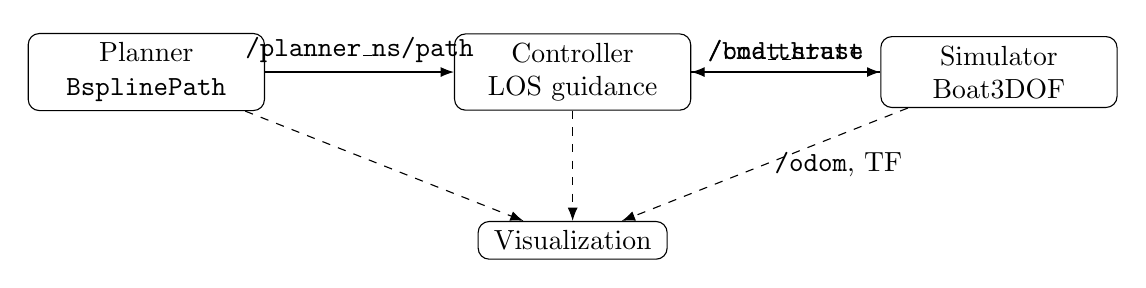
\begin{tikzpicture}[>=Latex,node distance=2.4cm]
    \node[draw,rounded corners,align=center,minimum width=3.0cm] (planner) {Planner\\\texttt{BsplinePath}};
    \node[draw,rounded corners,align=center,minimum width=3.0cm,right=of planner] (controller) {Controller\\LOS guidance};
    \node[draw,rounded corners,align=center,minimum width=3.0cm,right=of controller] (sim) {Simulator\\Boat3DOF};
    \node[draw,rounded corners,align=center,minimum width=2.4cm,below=1.4cm of controller] (viz) {Visualization};

    \draw[->] (planner) -- node[above] {\texttt{/planner\_ns/path}} (controller);
    \draw[->] (controller) -- node[above] {\texttt{/cmd\_thrust}} (sim);
    \draw[->] (sim) -- node[above] {\texttt{/boat\_state}} (controller);
    \draw[->,dashed] (sim) -- node[right] {\texttt{/odom}, TF} (viz);
    \draw[->,dashed] (planner) -- (viz);
    \draw[->,dashed] (controller) -- (viz);
  \end{tikzpicture}
  \caption{Data flow between the planner, controller, simulator, and visualization.}
  \label{fig:architecture}
\end{figure}

\section{Definitions}
\label{sec:definitions}
This section is the single source of truth for frames, symbols, and sign
conventions used throughout the document.

\subsection{ENU convention (world frame)}
\label{sec:enu_convention}
\paragraph{Purpose.}
Fix a single world-frame orientation so position, heading, and gravity signs are
consistent across models, plots, and code.

\paragraph{Assumptions.}
The world frame is locally tangent to Earth and treated as inertial over the
trajectory of interest; curvature and Coriolis effects are neglected.

\paragraph{Definitions.}
The inertial world frame $\{W\}$ follows the ENU convention with basis vectors
$\{\mathbf{e}_E,\mathbf{e}_N,\mathbf{e}_U\}$:
$+x_W$ points East, $+y_W$ points North, and $+z_W$ points Up. A position
vector in $\{W\}$ is $\mathbf{r}^W=[x,y,z]^\top$, where $z>0$ means above the
origin. All rotations follow the right-hand rule. The yaw angle $\psi$ is the
right-hand rotation about $+z_W$, so positive yaw rotates $+x_W$ toward $+y_W$
(counterclockwise when viewed from above).

\paragraph{Model statement.}
In planar motion, the ENU yaw convention implies the horizontal heading
direction
\[
  \hat{\mathbf{h}}^W =
  \begin{bmatrix}
    \cos\psi \\ \sin\psi \\ 0
  \end{bmatrix},
\]
so a positive $\psi$ rotates the East axis toward North in the horizontal plane.

\paragraph{Implementation mapping.}
State estimates, logged trajectories, and planner inputs store $x,y,z$ in ENU.
The kinematic updates in the simulator and tests (e.g.,
\texttt{src/na\_sim/test/test\_enu\_conventions.py}) interpret $\psi$ using the
counterclockwise ENU convention and use $\psi$ to map body-frame velocities
into the world frame consistent with the heading direction above.

\begin{figure}[h]
  \centering
  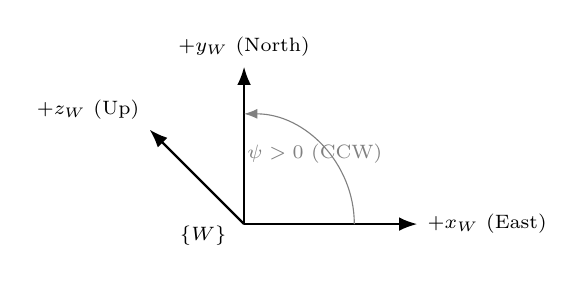
\begin{tikzpicture}[>=Latex,scale=1.0,every node/.style={font=\scriptsize}]
    \coordinate (O) at (0,0);
    \draw[->,thick] (O) -- (2.2,0) node[anchor=west] {$+x_W$ (East)};
    \draw[->,thick] (O) -- (0,2.0) node[anchor=south] {$+y_W$ (North)};
    \draw[->,thick] (O) -- (-1.2,1.2) node[anchor=south east] {$+z_W$ (Up)};
    \draw[->,gray] (1.4,0) arc[start angle=0,end angle=90,radius=1.4];
    \node[gray] at (0.9,0.9) {$\psi>0$ (CCW)};
    \node[anchor=north east] at (-0.1,0.1) {$\{W\}$};
  \end{tikzpicture}
  \caption{ENU world frame $\{W\}$: east-north-up axes and positive yaw about $+z_W$.}
  \label{fig:enu_axes}
\end{figure}

\subsection{Body frame (FLU)}
The simulator uses a world frame $\{W\}$ and a body frame $\{B\}$, corresponding
to ROS~2 \texttt{map} and \texttt{base\_link}, respectively. The body frame is
right-handed with $+x_B$ forward, $+y_B$ to port/left, and $+z_B$ upward (FLU).
This aligns the body axes with the ENU convention in \Cref{sec:enu_convention}.

\paragraph{Marine-convention note.}
This document and the codebase use the ROS ENU/FLU convention throughout.

\subsection{State, inputs, and generalized forces}
We split vessel pose and velocity using standard marine craft notation:
\begin{align*}
  \boldsymbol{\eta} &=
  \begin{bmatrix}
    x & y & z & \phi & \theta & \psi
  \end{bmatrix}^\top, &
  \boldsymbol{\nu} &=
  \begin{bmatrix}
    u & v & w & p & q & r
  \end{bmatrix}^\top,
\end{align*}
where $(x,y,z,\phi,\theta,\psi)$ are expressed in $\{W\}$ and $(u,v,w,p,q,r)$ in
$\{B\}$. The current simulator is planar (3~DOF) and uses:
\[
  \boldsymbol{\eta}_3 =
  \begin{bmatrix}
    x & y & \psi
  \end{bmatrix}^\top, \qquad
  \boldsymbol{\nu}_3 =
  \begin{bmatrix}
    u & v & r
  \end{bmatrix}^\top.
\]

The control input is a stern-mounted steerable rotor producing a thrust
magnitude $T$ and a steering angle $\delta$ relative to $+x_B$ (positive to
port/left).
Generalized forces and moments are collected in
$\boldsymbol{\tau}=[X,Y,Z,K,M,N]^\top$ (body frame). The planar simulator uses
$\boldsymbol{\tau}_3=[X,Y,N]^\top$.

\subsection{Units and core symbols}
\begin{table}[h]
  \centering
  \begin{tabular}{@{}llll@{}}
    \toprule
    Symbol & Meaning & Frame & Units \\
    \midrule
    $x,y,z$ & Position of the body origin & $\{W\}$ & \si{\meter} \\
    $\phi,\theta,\psi$ & Roll, pitch, yaw (ZYX) & $\{W\}$ & \si{\radian} \\
    $u,v,w$ & Linear velocity & $\{B\}$ & \si{\meter\per\second} \\
    $p,q,r$ & Angular velocity & $\{B\}$ & \si{\radian\per\second} \\
    $\mathbf{q}_{WB}$ & Unit quaternion, body-to-world & -- & -- \\
    $T$ & Thrust magnitude & $\{B\}$ & \si{\newton} \\
    $\delta$ & Steering angle (about $+z_B$) & $\{B\}$ & \si{\radian} \\
    $\ell$ & Rotor arm (rotor at $x_B=-\ell$) & $\{B\}$ & \si{\meter} \\
    $X,Y,Z$ & Forces & $\{B\}$ & \si{\newton} \\
    $K,M,N$ & Moments & $\{B\}$ & \si{\newton\meter} \\
    $m$ & Mass & -- & \si{\kilogram} \\
    $I_z$ & Yaw moment of inertia & -- & \si{\kilogram\meter\squared} \\
    \bottomrule
  \end{tabular}
  \caption{Core symbols and units used by the vessel models.}
  \label{tab:defs_units}
\end{table}

\subsection{Common vectors and matrices}
\begin{table}[h]
  \centering
  \begin{tabular}{@{}lll@{}}
    \toprule
    Name & Definition & Dimensions \\
    \midrule
    $\boldsymbol{\eta}$ & $[x,y,z,\phi,\theta,\psi]^\top$ & $6\times 1$ \\
    $\boldsymbol{\nu}$ & $[u,v,w,p,q,r]^\top$ & $6\times 1$ \\
    $\boldsymbol{\tau}$ & $[X,Y,Z,K,M,N]^\top$ & $6\times 1$ \\
    $\boldsymbol{\omega}$ & $[p,q,r]^\top$ & $3\times 1$ \\
    $\Delta\mathbf{q}$ & Expmap delta quaternion & $4\times 1$ \\
    $\boldsymbol{\phi}$ & Rotation vector, $\boldsymbol{\omega}\Delta t$ & $3\times 1$ \\
    $\mathbf{a}$ & Unit rotation axis, $\boldsymbol{\phi}/\|\boldsymbol{\phi}\|$ & $3\times 1$ \\
    $\boldsymbol{\xi}$ & Lie algebra coordinate for $SO(3)$ & $3\times 1$ \\
    $[\mathbf{a}]_\times$ & $\mathbf{a}\times\mathbf{b}=[\mathbf{a}]_\times\mathbf{b}$ & $3\times 3$ \\
    $\boldsymbol{\Omega}(\boldsymbol{\omega})$ & Quaternion kinematic matrix & $4\times 4$ \\
    $\mathbf{R}(\cdot)$ & Body-to-world rotation & $3\times 3$ \\
    $\mathbf{J}(\boldsymbol{\eta})$ & Kinematic transform in $\dot{\boldsymbol{\eta}}=\mathbf{J}\boldsymbol{\nu}$ & $6\times 6$ \\
    \bottomrule
  \end{tabular}
  \caption{Common vectors and matrices.}
  \label{tab:defs_common}
\end{table}

\subsection{Operators}
For $\mathbf{a}=[a_x,a_y,a_z]^\top$, define the cross-product (skew) operator:
\[
  [\mathbf{a}]_\times =
  \begin{bmatrix}
    0 & -a_z & a_y \\
    a_z & 0 & -a_x \\
    -a_y & a_x & 0
  \end{bmatrix}, \qquad
  \mathbf{a}\times\mathbf{b} = [\mathbf{a}]_\times \mathbf{b}.
\]
The matrix exponential $\exp([\mathbf{a}]_\times)$ maps the rotation vector
$\mathbf{a}$ to a rotation in $SO(3)$ (Rodrigues' formula), and is used in the
expmap update with $\mathbf{a}=\boldsymbol{\omega}\Delta t$. Note that the
exponential of a skew-symmetric matrix is computed via the matrix exponential
(Rodrigues), not elementwise.
An easy example is $\mathbf{a}=[0,0,\theta]^\top$:
\[
  [\mathbf{a}]_\times =
  \begin{bmatrix}
    0 & -\theta & 0 \\
    \theta & 0 & 0 \\
    0 & 0 & 0
  \end{bmatrix}, \qquad
  \exp([\mathbf{a}]_\times) =
  \begin{bmatrix}
    \cos\theta & -\sin\theta & 0 \\
    \sin\theta & \cos\theta & 0 \\
    0 & 0 & 1
  \end{bmatrix}.
\]

\subsection{Notation collisions}
The code uses $u$ for both surge velocity (a standard marine convention) and the
spline's internal unitless parameter. In the text we write the spline parameter
as $u_{\mathrm{spline}}$ when needed; the arc-length parameter is denoted $t$
(meters), consistent with \texttt{BSplinePath}. Time derivatives use dot
notation, e.g.\ $\dot{x}$.
\clearpage
\section{Planning (path generation)}
\subsection{Published message: \texttt{na\_msg/BsplinePath}}
The planner publishes a \texttt{BsplinePath} message consisting of parallel
arrays \texttt{ctrl\_x}, \texttt{ctrl\_y} (and \texttt{ctrl\_z}, currently always
zero). The controller requires:
\begin{itemize}
  \item at least 4 control points, and
  \item matching lengths for \texttt{ctrl\_x} and \texttt{ctrl\_y}.
\end{itemize}
The \texttt{closed} flag indicates whether indices wrap (closed loop) or clamp
at endpoints (open path). The message includes \texttt{degree} but the current
implementation always uses a uniform cubic spline, and therefore ignores
\texttt{degree}. The \texttt{start\_u} field provides an offset for the spline's
internal parameterization.

\subsection{Planner node (\texttt{planner\_node.py})}
The current ``planner'' is intentionally simple: it is a deterministic path
generator for closed-loop controller development. It publishes at a fixed timer
rate and selects a path using the parameter \texttt{path\_type}:
\begin{itemize}
  \item \texttt{CIRCLE}: a circle built from evenly spaced control points.
  \item \texttt{SQUARE\_SINUS}: a square-like loop with repeated corner points to
    adjust corner sharpness.
\end{itemize}

\subsection{Path alignment}
Before publishing, the planner aligns the path so runs start from a consistent
pose. The helper \texttt{\_align\_path\_to\_origin}:
\begin{enumerate}
  \item samples a closed spline preview,
  \item selects an ``anchor'' at approximately the lowest-$y$ sample,
  \item rotates the path so the local tangent points along $+x$, and
  \item translates the anchor to the origin.
\end{enumerate}
This keeps experiments repeatable across restarts.

\subsection{Uniform cubic B-spline representation}
The published control points are interpreted as a uniform cubic B-spline. The
code uses a unitless internal parameter $u_{\mathrm{spline}} = i + \tau$, where
$i=\lfloor u_{\mathrm{spline}} \rfloor$ and $\tau \in [0,1)$. The spline value is
\[
  \mathbf{C}(u_{\mathrm{spline}}) = b_0(\tau)\mathbf{P}_{i-1} + b_1(\tau)\mathbf{P}_{i}
  + b_2(\tau)\mathbf{P}_{i+1} + b_3(\tau)\mathbf{P}_{i+2},
\]
with basis functions:
\begin{align}
  b_0(\tau) &= \frac{-\tau^3 + 3\tau^2 - 3\tau + 1}{6}, &
  b_1(\tau) &= \frac{3\tau^3 - 6\tau^2 + 4}{6}, \\
  b_2(\tau) &= \frac{-3\tau^3 + 3\tau^2 + 3\tau + 1}{6}, &
  b_3(\tau) &= \frac{\tau^3}{6}.
\end{align}
For closed paths, indices wrap modulo $n$. For open paths, $u_{\mathrm{spline}}$
spans $[0,\,n-3]$ and clamps at the ends.

\subsection{Sampling and arc length}
\texttt{BSplinePath} samples the spline uniformly in $u_{\mathrm{spline}}$ and
accumulates Euclidean distances to approximate arc length $t$ (meters). The
sampled arrays provide fast conversions between $u_{\mathrm{spline}}$ and $t$.
The helper \texttt{samples\_from\_density} converts a \texttt{samples\_per\_meter}
tuning knob into a sample count by estimating the spline length from a coarse
preview.

\subsection{Planner parameters}
The planner currently exposes:
\begin{table}[h]
  \centering
  \begin{tabular}{@{}llll@{}}
    \toprule
    Parameter & Default & Units & Meaning \\
    \midrule
    \texttt{path\_type} & \texttt{SQUARE\_SINUS} & -- & Which demo path to publish \\
    \texttt{samples\_per\_meter} & 4.0 & \si{\per\meter} & Sampling density for preview + controller \\
    \bottomrule
  \end{tabular}
  \caption{Planner node parameters (see \texttt{planner\_node.py}).}
  \label{tab:planner_params}
\end{table}
\clearpage
\section{Control (LOS guidance)}
\subsection{Projection and Frenet frame}
The controller operates in the path's local Frenet frame, obtained by projecting
the boat position $(x,y)$ onto the spline. Projection is a two-stage process:
\begin{enumerate}
  \item Find the nearest sampled point (optionally within a window around a hint).
  \item Refine $u_{\mathrm{spline}}$ with a Gauss--Newton step along the spline tangent:
  \[
    \Delta u_{\mathrm{spline}} =
      \frac{(\mathbf{p}-\mathbf{C}(u_{\mathrm{spline}})) \cdot \mathbf{C}'(u_{\mathrm{spline}})}
      {\mathbf{C}'(u_{\mathrm{spline}})\cdot\mathbf{C}'(u_{\mathrm{spline}})}.
  \]
\end{enumerate}
The result provides a Frenet frame with unit tangent $\hat{\mathbf{t}}$,
unit normal $\hat{\mathbf{n}} = (-\hat{t}_y,\hat{t}_x)$ (left normal), and signed
cross-track error
\[
  cte = (\mathbf{p}-\mathbf{p}_{proj}) \cdot \hat{\mathbf{n}}.
\]
With this convention, $cte > 0$ means the boat is to the left of the path
tangent direction.
These geometric utilities in \texttt{na\_utils} use the ENU/FLU convention
directly when computing $\psi_{path}$.

\subsection{\texttt{ProjectionTracker}}
\texttt{ProjectionTracker} adds state to stabilize sequential projections:
\begin{itemize}
  \item It keeps the last arc-length projection $t$.
  \item It predicts forward progress using body velocities and heading, by
    projecting the inertial velocity onto the path tangent.
  \item It limits jumps via \texttt{max\_jump} and can enforce minimum forward
    progress when the along-track speed is positive.
\end{itemize}
This reduces projection snapping on self-intersections but does not eliminate
all ambiguity.

\subsection{LOS guidance law}
The controller follows a line-of-sight (LOS) guidance pattern:
\begin{enumerate}
  \item If no valid spline is available, publish $[0,0]$ and exit.
  \item Project $(x,y)$ onto the path to get $t$, tangent, normal, and $cte$.
  \item Compute the path heading $\psi_{path}$ from the tangent; under ENU this
    uses $\psi_{path} = \arctan2(t_y, t_x)$, and if the tangent norm is near
    zero, $\psi_{path}=0$.
  \item Choose a lookahead distance $L$ and advance to $t_{target}=t+L$.
  \item Compute desired heading
    \[
      \psi_d = \mathrm{wrap}\left(\psi_{path} - \arctan2(cte, L)\right).
    \]
  \item Apply a PD law on heading error with saturation:
    \[
      \delta = \mathrm{sat}\left(-k_p\,\mathrm{wrap}(\psi_d-\psi) + k_d\,r,\;\delta_{\max}\right).
    \]
  \item Thrust is constant: $T=\mathrm{sat}(T_0, T_{\max})$.
\end{enumerate}
The steering sign is consistent with the simulator's moment convention: positive
$\delta$ produces a negative yaw moment, so the proportional term uses a leading
minus sign, while the damping term uses $+k_d r$ to oppose yaw-rate excursions.

\subsection{Configuration parameters}
Default parameters live in \texttt{src/na\_launch/config/sim\_controller\_params.yaml}.
\texttt{config\_path} can override the YAML file for both simulator and controller.

\subsection{Controller parameters}
\begin{table}[h]
  \centering
  \begin{tabular}{@{}llll@{}}
    \toprule
    Parameter & Default & Units & Meaning \\
    \midrule
    \texttt{path\_topic} & \texttt{/planner\_ns/path} & -- & BsplinePath source \\
    \texttt{lookahead} & 4.0 & \si{\meter} & LOS lookahead distance \\
    \texttt{base\_thrust} & 15.0 & \si{\newton} & Constant thrust command \\
    \texttt{heading\_kp} & 2.0 & -- & Heading proportional gain \\
    \texttt{heading\_kd} & 0.5 & \si{\second} & Yaw-rate damping gain \\
    \texttt{max\_thrust} & 30.0 & \si{\newton} & Thrust saturation \\
    \texttt{max\_delta} & 1.570796 & \si{\radian} & Steering saturation \\
    \texttt{samples\_per\_meter} & 4.0 & \si{\per\meter} & B-spline sample density \\
    \texttt{max\_proj\_jump} & 0.2 & \si{\meter} & Projection jump limit \\
    \bottomrule
  \end{tabular}
  \caption{Controller tuning parameters and defaults.}
  \label{tab:controller_params}
\end{table}

\subsection{Examples and edge cases}
Figures in this section are generated from the same B-spline utilities used by
the controller. To refresh them, run
\texttt{latex/scripts/generate\_figures.py} and update the inline TikZ blocks in
this file.

\subsubsection{Example: closed-loop LOS tracking}
\Cref{fig:los_example} illustrates the projection, cross-track error, and
lookahead target on a closed spline generated from the same projection code.
\begin{figure}[h]
  \centering
% Auto-generated by latex/scripts/generate_figures.py
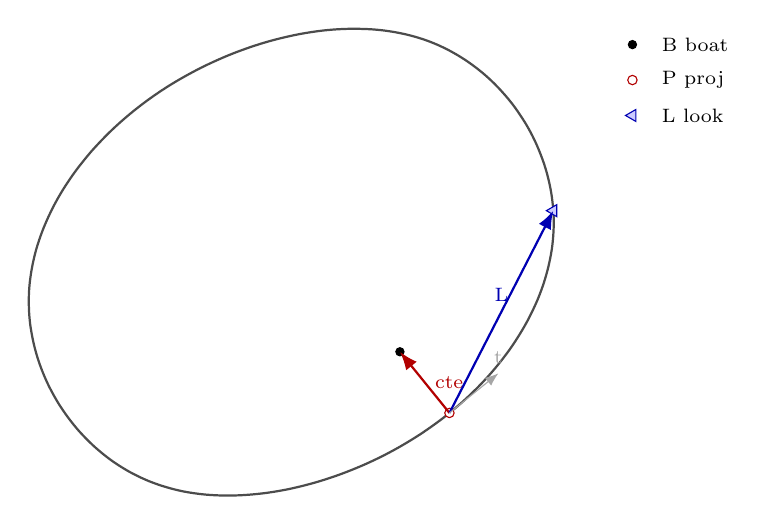
\begin{tikzpicture}[>=Latex,scale=1.0,every node/.style={font=\scriptsize}]
  \tikzset{
    path/.style={thick,black!70},
    cte/.style={red!70!black,thick,->},
    look/.style={blue!70!black,thick,->},
    tan/.style={gray!70,->},
    boat/.style={circle,fill=black,inner sep=1.2pt},
    proj/.style={circle,draw=red!70!black,fill=white,inner sep=1.2pt},
    lookahead/.style={regular polygon,regular polygon sides=3,draw=blue!70!black,fill=blue!20,minimum size=5pt,inner sep=0pt,rotate=90}
  }
  \draw[path] plot [smooth cycle] coordinates { (0.333,0.667) (0.471,0.626) (0.612,0.592) (0.756,0.567) (0.903,0.549) (1.053,0.539) (1.205,0.536) (1.359,0.540) (1.515,0.551) (1.672,0.568) (1.829,0.592) (1.987,0.622) (2.145,0.659) (2.302,0.701) (2.459,0.749) (2.615,0.803) (2.769,0.862) (2.922,0.926) (3.072,0.995) (3.220,1.069) (3.365,1.148) (3.506,1.231) (3.644,1.318) (3.778,1.410) (3.908,1.505) (4.033,1.605) (4.154,1.707) (4.270,1.814) (4.381,1.923) (4.487,2.035) (4.587,2.150) (4.682,2.268) (4.772,2.388) (4.855,2.511) (4.932,2.635) (5.004,2.762) (5.068,2.890) (5.127,3.020) (5.178,3.151) (5.222,3.283) (5.259,3.416) (5.289,3.550) (5.312,3.685) (5.326,3.820) (5.333,3.955) (5.332,4.090) (5.322,4.225) (5.305,4.360) (5.280,4.493) (5.248,4.625) (5.208,4.756) (5.161,4.884) (5.108,5.010) (5.048,5.133) (4.981,5.253) (4.907,5.369) (4.828,5.482) (4.742,5.590) (4.651,5.693) (4.554,5.792) (4.452,5.885) (4.344,5.972) (4.232,6.053) (4.114,6.128) (3.992,6.196) (3.865,6.257) (3.734,6.310) (3.598,6.355) (3.459,6.392) (3.317,6.421) (3.171,6.443) (3.022,6.457) (2.871,6.463) (2.718,6.463) (2.563,6.456) (2.407,6.442) (2.250,6.421) (2.092,6.394) (1.934,6.360) (1.776,6.321) (1.619,6.276) (1.463,6.225) (1.308,6.169) (1.154,6.107) (1.003,6.040) (0.854,5.969) (0.708,5.892) (0.564,5.811) (0.424,5.726) (0.288,5.636) (0.157,5.543) (0.029,5.445) (-0.094,5.344) (-0.212,5.240) (-0.326,5.132) (-0.434,5.021) (-0.538,4.908) (-0.635,4.791) (-0.728,4.672) (-0.814,4.551) (-0.895,4.427) (-0.969,4.302) (-1.037,4.174) (-1.098,4.045) (-1.153,3.915) (-1.201,3.783) (-1.242,3.651) (-1.275,3.517) (-1.301,3.383) (-1.320,3.248) (-1.331,3.113) (-1.333,2.977) (-1.328,2.842) (-1.315,2.707) (-1.293,2.573) (-1.265,2.441) (-1.229,2.309) (-1.186,2.180) (-1.136,2.053) (-1.079,1.928) (-1.015,1.807) (-0.945,1.688) (-0.868,1.574) (-0.786,1.464) (-0.698,1.358) (-0.603,1.257) (-0.504,1.161) (-0.399,1.071) (-0.289,0.986) (-0.173,0.908) (-0.054,0.837) (0.071,0.773) (0.200,0.716) (0.333,0.667) };
  \coordinate (boat) at (3.380,2.362);
  \coordinate (proj) at (4.009,1.585);
  \coordinate (target) at (5.328,4.154);
  \coordinate (tan) at (4.631,2.088);
  \node[boat] at (boat) {};
  \node[proj] at (proj) {};
  \node[lookahead] at (target) {};
  \draw[cte] (proj) -- (boat) node[midway,right] {cte};
  \draw[look] (proj) -- (target) node[midway,above] {L};
  \draw[tan] (proj) -- (tan) node[above] {t};
  \node[boat] at (6.333,6.263) {};
  \node[anchor=west] at (6.583,6.263) {B boat};
  \node[proj] at (6.333,5.813) {};
  \node[anchor=west] at (6.583,5.813) {P proj};
  \node[lookahead] at (6.333,5.363) {};
  \node[anchor=west] at (6.583,5.363) {L look};
\end{tikzpicture}
  \caption{LOS tracking geometry on a closed spline generated from the path utilities (B: boat, P: projection, L: lookahead).}
  \label{fig:los_example}
\end{figure}

\subsubsection{Example: open path end behavior}
\Cref{fig:open_end} shows an open path with the vessel near the end. The
lookahead point clamps at the end of the spline; there is no wrap-around.
\begin{figure}[h]
  \centering
% Auto-generated by latex/scripts/generate_figures.py
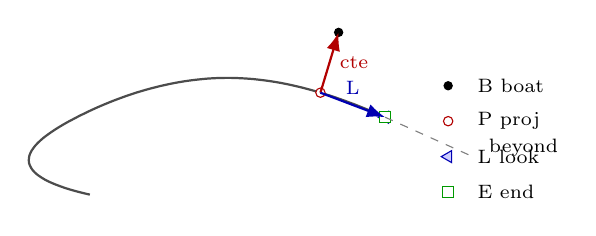
\begin{tikzpicture}[>=Latex,scale=1.0,every node/.style={font=\scriptsize}]
  \tikzset{
    path/.style={thick,black!70},
    cte/.style={red!70!black,thick,->},
    look/.style={blue!70!black,thick,->},
    boat/.style={circle,fill=black,inner sep=1.2pt},
    proj/.style={circle,draw=red!70!black,fill=white,inner sep=1.2pt},
    lookahead/.style={regular polygon,regular polygon sides=3,draw=blue!70!black,fill=blue!20,minimum size=5pt,inner sep=0pt,rotate=90},
    endpt/.style={rectangle,draw=green!60!black,fill=white,minimum size=4pt,inner sep=0pt}
  }
  \draw[path] plot [smooth] coordinates { (-2.250,0.117) (-2.358,0.143) (-2.457,0.169) (-2.547,0.196) (-2.628,0.224) (-2.701,0.252) (-2.766,0.280) (-2.823,0.309) (-2.872,0.339) (-2.914,0.368) (-2.949,0.398) (-2.977,0.429) (-2.998,0.459) (-3.013,0.490) (-3.023,0.521) (-3.026,0.552) (-3.024,0.583) (-3.018,0.614) (-3.006,0.645) (-2.989,0.677) (-2.968,0.708) (-2.944,0.739) (-2.915,0.770) (-2.883,0.801) (-2.848,0.832) (-2.809,0.862) (-2.768,0.892) (-2.725,0.922) (-2.679,0.952) (-2.632,0.981) (-2.583,1.010) (-2.532,1.039) (-2.481,1.066) (-2.428,1.094) (-2.376,1.121) (-2.322,1.147) (-2.269,1.173) (-2.215,1.198) (-2.160,1.223) (-2.105,1.247) (-2.050,1.270) (-1.994,1.293) (-1.938,1.315) (-1.882,1.336) (-1.825,1.357) (-1.769,1.377) (-1.711,1.396) (-1.654,1.415) (-1.596,1.432) (-1.538,1.449) (-1.480,1.465) (-1.421,1.480) (-1.363,1.495) (-1.304,1.508) (-1.245,1.521) (-1.186,1.533) (-1.126,1.544) (-1.067,1.554) (-1.007,1.563) (-0.947,1.571) (-0.887,1.578) (-0.827,1.584) (-0.767,1.590) (-0.707,1.594) (-0.647,1.597) (-0.587,1.599) (-0.527,1.600) (-0.467,1.600) (-0.406,1.599) (-0.346,1.596) (-0.286,1.593) (-0.226,1.589) (-0.166,1.584) (-0.105,1.577) (-0.045,1.570) (0.015,1.562) (0.075,1.553) (0.135,1.543) (0.196,1.532) (0.256,1.520) (0.316,1.507) (0.376,1.493) (0.436,1.479) (0.497,1.463) (0.557,1.447) (0.617,1.430) (0.677,1.413) (0.737,1.394) (0.798,1.375) (0.858,1.355) (0.918,1.334) (0.978,1.313) (1.038,1.290) (1.099,1.268) (1.159,1.244) (1.219,1.220) (1.279,1.196) (1.339,1.170) (1.400,1.144) (1.460,1.118) (1.500,1.100) };
  \coordinate (boat) at (0.909,2.178);
  \coordinate (proj) at (0.678,1.412);
  \coordinate (target) at (1.500,1.100);
  \coordinate (endpt) at (1.500,1.100);
  \coordinate (beyond) at (2.594,0.608);
  \node[boat] at (boat) {};
  \node[proj] at (proj) {};
  \node[lookahead] at (target) {};
  \node[endpt] at (endpt) {};
  \draw[cte] (proj) -- (boat) node[midway,right] {cte};
  \draw[look] (proj) -- (target) node[midway,above] {L};
  \draw[dashed,gray] (endpt) -- (beyond);
  \node[anchor=west] at (2.694,0.708) {beyond};
  \node[boat] at (2.300,1.500) {};
  \node[anchor=west] at (2.550,1.500) {B boat};
  \node[proj] at (2.300,1.050) {};
  \node[anchor=west] at (2.550,1.050) {P proj};
  \node[lookahead] at (2.300,0.600) {};
  \node[anchor=west] at (2.550,0.600) {L look};
  \node[endpt] at (2.300,0.150) {};
  \node[anchor=west] at (2.550,0.150) {E end};
\end{tikzpicture}
  \caption{Open-path end behavior: \texttt{advance\_t} clamps instead of wrapping (B: boat, P: projection, L: lookahead, E: end).}
  \label{fig:open_end}
\end{figure}

\subsubsection{Edge case: sparse sampling}
\Cref{fig:sampling_density} compares a dense spline sample to a coarse sample
count. Sparse samples reduce projection accuracy and can create large $cte$
discontinuities.
\begin{figure}[h]
  \centering
% Auto-generated by latex/scripts/generate_figures.py
\begin{tikzpicture}[>=Latex,scale=0.95,every node/.style={font=\scriptsize}]
  \tikzset{
    finepath/.style={thick,black!70},
    coarsepath/.style={orange!80!black,dashed},
    coarsept/.style={circle,draw=orange!80!black,fill=orange!40,inner sep=0.6pt}
  }
  \draw[finepath] plot [smooth cycle] coordinates { (-3.667,0.000) (-3.664,0.100) (-3.657,0.200) (-3.645,0.300) (-3.628,0.400) (-3.606,0.499) (-3.581,0.597) (-3.551,0.695) (-3.517,0.791) (-3.478,0.887) (-3.436,0.982) (-3.391,1.075) (-3.341,1.167) (-3.288,1.257) (-3.232,1.346) (-3.172,1.433) (-3.109,1.518) (-3.044,1.601) (-2.975,1.682) (-2.904,1.761) (-2.830,1.837) (-2.753,1.911) (-2.674,1.982) (-2.593,2.051) (-2.510,2.117) (-2.424,2.181) (-2.337,2.242) (-2.248,2.301) (-2.158,2.357) (-2.066,2.411) (-1.972,2.462) (-1.877,2.511) (-1.782,2.557) (-1.685,2.601) (-1.587,2.642) (-1.489,2.680) (-1.390,2.716) (-1.290,2.750) (-1.190,2.781) (-1.090,2.810) (-0.990,2.836) (-0.890,2.859) (-0.789,2.880) (-0.689,2.899) (-0.589,2.915) (-0.489,2.928) (-0.388,2.939) (-0.288,2.948) (-0.188,2.954) (-0.088,2.957) (0.013,2.958) (0.113,2.957) (0.213,2.953) (0.313,2.946) (0.414,2.937) (0.514,2.925) (0.614,2.911) (0.714,2.895) (0.815,2.875) (0.915,2.854) (1.015,2.830) (1.115,2.803) (1.215,2.774) (1.315,2.742) (1.415,2.708) (1.513,2.671) (1.612,2.632) (1.709,2.590) (1.806,2.546) (1.901,2.499) (1.996,2.450) (2.089,2.398) (2.180,2.343) (2.271,2.287) (2.359,2.227) (2.446,2.165) (2.531,2.101) (2.613,2.034) (2.694,1.965) (2.772,1.893) (2.848,1.818) (2.922,1.741) (2.992,1.662) (3.060,1.581) (3.125,1.497) (3.187,1.411) (3.246,1.324) (3.302,1.235) (3.354,1.144) (3.402,1.052) (3.447,0.958) (3.488,0.863) (3.526,0.767) (3.559,0.670) (3.588,0.572) (3.612,0.474) (3.632,0.375) (3.648,0.275) (3.659,0.175) (3.665,0.075) (3.667,-0.025) (3.663,-0.125) (3.654,-0.225) (3.641,-0.325) (3.623,-0.424) (3.600,-0.523) (3.574,-0.621) (3.543,-0.719) (3.507,-0.815) (3.468,-0.911) (3.425,-1.005) (3.379,-1.098) (3.328,-1.189) (3.274,-1.279) (3.217,-1.368) (3.157,-1.454) (3.093,-1.539) (3.027,-1.622) (2.957,-1.702) (2.885,-1.780) (2.811,-1.856) (2.734,-1.929) (2.654,-2.000) (2.572,-2.068) (2.488,-2.133) (2.403,-2.197) (2.315,-2.257) (2.226,-2.315) (2.135,-2.371) (2.042,-2.424) (1.949,-2.474) (1.854,-2.523) (1.758,-2.568) (1.660,-2.611) (1.563,-2.652) (1.464,-2.690) (1.365,-2.725) (1.265,-2.758) (1.165,-2.789) (1.065,-2.817) (0.965,-2.842) (0.865,-2.865) (0.764,-2.885) (0.664,-2.903) (0.564,-2.919) (0.464,-2.931) (0.363,-2.942) (0.263,-2.950) (0.163,-2.955) (0.063,-2.958) (-0.038,-2.958) (-0.138,-2.956) (-0.238,-2.951) (-0.338,-2.944) (-0.439,-2.934) (-0.539,-2.922) (-0.639,-2.907) (-0.739,-2.890) (-0.840,-2.870) (-0.940,-2.848) (-1.040,-2.823) (-1.140,-2.796) (-1.240,-2.766) (-1.340,-2.734) (-1.439,-2.699) (-1.538,-2.661) (-1.636,-2.621) (-1.733,-2.579) (-1.830,-2.534) (-1.925,-2.487) (-2.019,-2.437) (-2.112,-2.384) (-2.203,-2.329) (-2.293,-2.272) (-2.381,-2.212) (-2.467,-2.149) (-2.552,-2.084) (-2.634,-2.017) (-2.714,-1.947) (-2.792,-1.874) (-2.867,-1.799) (-2.940,-1.722) (-3.010,-1.642) (-3.077,-1.560) (-3.141,-1.476) (-3.202,-1.390) (-3.260,-1.302) (-3.315,-1.212) (-3.366,-1.121) (-3.414,-1.028) (-3.458,-0.934) (-3.498,-0.839) (-3.534,-0.743) (-3.566,-0.646) (-3.594,-0.548) (-3.618,-0.449) (-3.637,-0.350) (-3.651,-0.250) (-3.661,-0.150) (-3.666,-0.050) (-3.667,0.000) };
  \draw[coarsepath] plot [smooth cycle] coordinates { (-3.667,0.000) (-3.555,0.683) (-3.246,1.325) (-2.781,1.884) (-2.202,2.330) (-1.548,2.657) (-0.862,2.865) (-0.172,2.955) (0.517,2.925) (1.207,2.776) (1.882,2.509) (2.503,2.122) (3.030,1.617) (3.422,1.011) (3.638,0.344) (3.638,-0.344) (3.422,-1.011) (3.030,-1.617) (2.503,-2.122) (1.882,-2.509) (1.207,-2.776) (0.517,-2.925) (-0.172,-2.955) (-0.862,-2.865) (-1.548,-2.657) (-2.202,-2.330) (-2.781,-1.884) (-3.246,-1.325) (-3.555,-0.683) (-3.667,0.000) };
  \foreach \p in {(-3.667,0.000), (-3.555,0.683), (-3.246,1.325), (-2.781,1.884), (-2.202,2.330), (-1.548,2.657), (-0.862,2.865), (-0.172,2.955), (0.517,2.925), (1.207,2.776), (1.882,2.509), (2.503,2.122), (3.030,1.617), (3.422,1.011), (3.638,0.344), (3.638,-0.344), (3.422,-1.011), (3.030,-1.617), (2.503,-2.122), (1.882,-2.509), (1.207,-2.776), (0.517,-2.925), (-0.172,-2.955), (-0.862,-2.865), (-1.548,-2.657), (-2.202,-2.330), (-2.781,-1.884), (-3.246,-1.325), (-3.555,-0.683), (-3.667,0.000)} { \node[coarsept] at \p {}; }
  \draw[finepath] (3.367,2.758) -- (3.967,2.758);
  \node[anchor=west] at (4.317,2.758) {fine path};
  \draw[coarsepath] (3.367,2.308) -- (3.967,2.308);
  \node[anchor=west] at (4.317,2.308) {coarse path};
  \node[coarsept] at (3.667,1.858) {};
  \node[anchor=west] at (4.317,1.858) {samples};
\end{tikzpicture}
  \caption{Effect of low sampling density on the spline representation (coarse samples shown as points).}
  \label{fig:sampling_density}
\end{figure}

\subsubsection{Expected behavior}
\begin{itemize}
  \item Fewer than 4 control points or mismatched \texttt{ctrl\_x}/\texttt{ctrl\_y} arrays:
    controller rejects the path, outputs $[0,0]$, and resets projection history.
  \item Very low \texttt{samples\_per\_meter} (or non-positive values): the spline is
    still built but with coarse sampling, which degrades projection accuracy (see
    \Cref{fig:sampling_density}).
  \item Self-intersections or tight loops: multiple projections can be locally optimal.
    \texttt{max\_proj\_jump} helps, but jumps are still possible with sharp geometry.
  \item Tangent norm near zero (repeated control points): heading defaults to 0,
    so steering may be arbitrary until geometry improves.
  \item Extremely small lookahead: high steering activity and oscillation.
    Extremely large lookahead: slow convergence and large steady-state $cte$.
\end{itemize}
\clearpage
\section{Simulator}
\subsection{Vessel dynamics (implemented: 3~DOF)}
\subsubsection{Assumptions}
\begin{itemize}
  \item Planar motion: $z=\phi=\theta=0$ and $w=p=q=0$.
  \item Constant mass properties with the body frame origin at the center of
    gravity (CG).
  \item Calm water: no current, wind, or wave loads.
  \item Hydrodynamics captured by low-order damping terms.
\end{itemize}

\subsubsection{Purpose}
Given state $\mathbf{x}=[x,y,\psi,u,v,r]^\top$ and actuator inputs $(T,\delta)$,
compute $\dot{\mathbf{x}}$ for time integration in \texttt{sim\_node.py}.

\subsubsection{Model}
Collect pose and velocity as $\boldsymbol{\eta}_3=[x,y,\psi]^\top$ and
$\boldsymbol{\nu}_3=[u,v,r]^\top$. The kinematics are:
\[
  \dot{\boldsymbol{\eta}}_3 = \mathbf{J}(\psi)\boldsymbol{\nu}_3, \qquad
  \mathbf{J}(\psi) =
  \begin{bmatrix}
    \cos\psi & -\sin\psi & 0 \\
    \sin\psi &  \cos\psi & 0 \\
    0         &  0        & 1
  \end{bmatrix},
\]
which expands to:
\begin{align}
  \dot{x} &= u\cos\psi - v\sin\psi, \\
  \dot{y} &= u\sin\psi + v\cos\psi, \\
  \dot{\psi} &= r.
\end{align}

\paragraph{Actuation mapping}
The steerable rotor produces:
\begin{align}
  X &= T\cos\delta, &
  Y &= T\sin\delta, &
  N &= -\ell\,Y = -\ell\,T\sin\delta,
\end{align}
and the generalized input is $\boldsymbol{\tau}_3=[X,Y,N]^\top$.
With ENU/FLU conventions, $\delta>0$ (port/left) implies $N<0$ and a clockwise
yaw response ($r<0$).

\paragraph{Dynamics (Fossen-style structure)}
The planar equations are written in the standard marine craft form:
\[
  \mathbf{M}_3\dot{\boldsymbol{\nu}}_3 +
  \mathbf{C}_3(\boldsymbol{\nu}_3)\boldsymbol{\nu}_3 +
  \mathbf{d}_3(\boldsymbol{\nu}_3) = \boldsymbol{\tau}_3,
\]
with:
\[
  \mathbf{M}_3 = \mathrm{diag}(m,\,m,\,I_z), \qquad
  \mathbf{C}_3(\boldsymbol{\nu}_3) =
  \begin{bmatrix}
    0 & 0 & -m v \\
    0 & 0 &  m u \\
    m v & -m u & 0
  \end{bmatrix},
\]
and damping vector:
\[
  \mathbf{d}_3(\boldsymbol{\nu}_3) =
  \begin{bmatrix}
    X_u u + X_{uu}|u|u \\
    Y_v v + Y_r r \\
    N_v v + N_r r
  \end{bmatrix}.
\]
Solving for $\dot{\boldsymbol{\nu}}_3$ yields:
\begin{align}
  \dot{u} &= \frac{1}{m}\!\left(X - X_u u - X_{uu}|u|u + mvr\right), \\
  \dot{v} &= \frac{1}{m}\!\left(Y - Y_v v - Y_r r - mur\right), \\
  \dot{r} &= \frac{1}{I_z}\!\left(N - N_v v - N_r r\right).
\end{align}

\subsubsection{Implementation mapping}
\texttt{Boat3DOF.dynamics()} in \texttt{src/na\_sim/na\_sim/Boat3DOF.py} evaluates
the kinematics, computes $(X,Y,N)$ from $(T,\delta)$, and applies the three
equations above to return $\dot{\mathbf{x}}$.

\subsection{Six degree of freedom marine craft model (Fossen, upgrade path)}
\subsubsection{Assumptions}
\begin{itemize}
  \item The body frame origin is at the CG unless stated otherwise.
  \item Mass properties are constant in time.
  \item Added mass is treated as constant (or slowly varying) for implementation.
  \item Hydrodynamic forces depend on the velocity relative to the water.
  \item Environmental loads are grouped in $\boldsymbol{\tau}_{\mathrm{env}}$.
\end{itemize}

\subsubsection{Purpose}
This subsection states the standard 6~DOF model used in Fossen-style marine
craft simulation and matches the implementation in
\texttt{src/na\_sim/na\_sim/fossen.py} (\texttt{Fossen6DOF}).

\subsubsection{Kinematics}
Let $\boldsymbol{\eta}=[x,y,z,\phi,\theta,\psi]^\top$ and
$\boldsymbol{\nu}=[u,v,w,p,q,r]^\top$ as defined in \Cref{sec:definitions}. The
6~DOF kinematics are:
\begin{equation}
  \dot{\boldsymbol{\eta}} = \mathbf{J}(\boldsymbol{\eta})\boldsymbol{\nu}, \qquad
  \mathbf{J}(\boldsymbol{\eta}) =
  \begin{bmatrix}
    \mathbf{R}(\phi,\theta,\psi) & \mathbf{0} \\
    \mathbf{0} & \mathbf{T}(\phi,\theta)
  \end{bmatrix}.
  \label{eq:fossen-kinematics-euler}
\end{equation}
Using a $ZYX$ (roll--pitch--yaw) convention,
$\mathbf{R}(\phi,\theta,\psi)=\mathbf{R}_z(\psi)\mathbf{R}_y(\theta)\mathbf{R}_x(\phi)$
maps body linear velocity to world velocity. Define $c_\alpha=\cos\alpha$ and
$s_\alpha=\sin\alpha$. Then:
\begin{equation}
  \mathbf{R}(\phi,\theta,\psi) =
  \begin{bmatrix}
    c_\psi c_\theta &
      c_\psi s_\theta s_\phi - s_\psi c_\phi &
      c_\psi s_\theta c_\phi + s_\psi s_\phi \\
    s_\psi c_\theta &
      s_\psi s_\theta s_\phi + c_\psi c_\phi &
      s_\psi s_\theta c_\phi - c_\psi s_\phi \\
    -s_\theta &
      c_\theta s_\phi &
      c_\theta c_\phi
  \end{bmatrix}.
  \label{eq:fossen-rotation-euler}
\end{equation}
The matrix
$\mathbf{T}(\phi,\theta)$ maps body angular velocity
$\boldsymbol{\omega}=[p,q,r]^\top$ to Euler angle rates:
\begin{equation}
  \begin{bmatrix}
    \dot{\phi} \\ \dot{\theta} \\ \dot{\psi}
  \end{bmatrix}
  =
  \mathbf{T}(\phi,\theta)
  \begin{bmatrix}
    p \\ q \\ r
  \end{bmatrix}, \qquad
  \mathbf{T}(\phi,\theta) =
  \begin{bmatrix}
    1 & \sin\phi\tan\theta & \cos\phi\tan\theta \\
    0 & \cos\phi & -\sin\phi \\
    0 & \sin\phi/\cos\theta & \cos\phi/\cos\theta
  \end{bmatrix}.
  \label{eq:fossen-euler-rate-map}
\end{equation}
The mapping is singular at $\cos\theta=0$.

\subsubsection{Attitude representation on $SO(3)$}
Euler angles are compact and match many marine references, but the
$\mathbf{T}(\phi,\theta)$ mapping becomes singular at $\theta=\pm\pi/2$.
Surface-vessel motion typically has small roll/pitch, so Euler angles are often
acceptable. For general 6~DOF simulation and ROS~2 integration, unit quaternions
are typically the most robust choice.

Let $\mathbf{q}_{WB}\in\mathbb{R}^4$ be a unit quaternion representing the
rotation from $\{B\}$ to $\{W\}$, with components
$\mathbf{q}_{WB}=[q_w,q_x,q_y,q_z]^\top$. Replace the Euler-angle kinematics by:
\begin{equation}
  \begin{aligned}
    \dot{\mathbf{p}} &=
    \mathbf{R}(\mathbf{q}_{WB})\mathbf{v}, \\
    \dot{\mathbf{q}}_{WB} &=
    \frac{1}{2}\,\boldsymbol{\Omega}(\boldsymbol{\omega})\mathbf{q}_{WB}, \\
    \boldsymbol{\Omega}(\boldsymbol{\omega}) &=
    \begin{bmatrix}
      0 & -p & -q & -r \\
      p & 0 & r & -q \\
      q & -r & 0 & p \\
      r & q & -p & 0
    \end{bmatrix}.
  \end{aligned}
  \label{eq:fossen-kinematics-quat}
\end{equation}
where $\mathbf{p}=[x,y,z]^\top$ is the world position, $\mathbf{v}=[u,v,w]^\top$
is the body linear velocity, and $\boldsymbol{\omega}=[p,q,r]^\top$ is the body
angular velocity from $\boldsymbol{\nu}$. Numerical
integration should renormalize $\mathbf{q}_{WB}$ to unit length.

The corresponding rotation matrix $\mathbf{R}(\mathbf{q}_{WB})$ is:
\begin{equation}
  \mathbf{R}(\mathbf{q}_{WB}) =
  \begin{bmatrix}
    1 - 2(q_y^2+q_z^2) & 2(q_x q_y - q_z q_w) & 2(q_x q_z + q_y q_w) \\
    2(q_x q_y + q_z q_w) & 1 - 2(q_x^2+q_z^2) & 2(q_y q_z - q_x q_w) \\
    2(q_x q_z - q_y q_w) & 2(q_y q_z + q_x q_w) & 1 - 2(q_x^2+q_y^2)
  \end{bmatrix}.
  \label{eq:fossen-rotation-quat}
\end{equation}

The Euler-angle and quaternion kinematics are consistent when they use the same
body-rate $\boldsymbol{\omega}$. The Euler form uses
$\dot{\boldsymbol{\eta}}=\mathbf{J}(\boldsymbol{\eta})\boldsymbol{\nu}$ with the
mapping $\dot{\boldsymbol{\Theta}}=\mathbf{T}(\phi,\theta)\boldsymbol{\omega}$,
while the quaternion form uses
$\dot{\mathbf{q}}_{WB}=\tfrac{1}{2}\boldsymbol{\Omega}(\boldsymbol{\omega})\mathbf{q}_{WB}$
and $\dot{\mathbf{p}}=\mathbf{R}(\mathbf{q}_{WB})\mathbf{v}$. For any set of
Euler angles $(\phi,\theta,\psi)$, the rotation matrix
$\mathbf{R}(\phi,\theta,\psi)$ equals $\mathbf{R}(\mathbf{q}_{WB})$ for the
equivalent unit quaternion, so the translational kinematics are identical away
from the Euler singularity at $\cos\theta=0$.

If a rotation-matrix state is preferred, one can integrate
$\dot{\mathbf{R}}=\mathbf{R}[\boldsymbol{\omega}]_\times$ and periodically
re-orthonormalize $\mathbf{R}$, or use a Lie-group update
$\mathbf{R}_{k+1}=\mathbf{R}_k\exp([\boldsymbol{\omega}\Delta t]_\times)$.

ROS~2 messages store quaternions as $(x,y,z,w)$.
Integrator theory (Euler, RK4, expmap, RKMK) is summarized in
\Cref{app:integrators} with an equation-by-equation mapping to the 6~DOF
implementation in \Cref{app:fossen-map}. The key update formulas are
Euler (\Cref{eq:euler}), RK4 (\Cref{eq:rk4}), and the expmap step
(\Cref{eq:expmap-dq,eq:expmap-update}).

\subsubsection{Dynamics}
The standard 6~DOF equations of motion in a body-fixed frame are:
\[
  \mathbf{M}\dot{\boldsymbol{\nu}} +
  \mathbf{C}(\boldsymbol{\nu})\boldsymbol{\nu} +
  \mathbf{D}(\boldsymbol{\nu})\boldsymbol{\nu} +
  \mathbf{g}(\boldsymbol{\eta})
  = \boldsymbol{\tau} + \boldsymbol{\tau}_{\mathrm{env}}.
\]
The terms are:
\begin{itemize}
  \item $\mathbf{M}=\mathbf{M}_{RB}+\mathbf{M}_A$: rigid-body and added-mass
    inertia (symmetric positive definite in typical operating regimes).
  \item $\mathbf{C}(\boldsymbol{\nu})=\mathbf{C}_{RB}(\boldsymbol{\nu})+\mathbf{C}_A(\boldsymbol{\nu})$:
    Coriolis/centripetal matrices associated with $\mathbf{M}_{RB}$ and
    $\mathbf{M}_A$.
  \item $\mathbf{D}(\boldsymbol{\nu})$: hydrodynamic damping (often split into
    linear and quadratic components).
  \item $\mathbf{g}(\boldsymbol{\eta})$: restoring forces and moments from
    gravity and buoyancy.
  \item $\boldsymbol{\tau}$: actuator generalized forces/moments in the body frame.
  \item $\boldsymbol{\tau}_{\mathrm{env}}$: environmental loads (wind, waves,
    current-induced loads, etc.).
\end{itemize}

\paragraph{Relative velocity and current}
Hydrodynamic terms (added mass and damping) depend on the velocity relative to
the water. Let $\mathbf{v}_c^W\in\mathbb{R}^3$ be the water current expressed in
the world frame and assume it has no angular component. Define:
\[
  \mathbf{v}_c^B = \mathbf{R}^\top \mathbf{v}_c^W, \qquad
  \boldsymbol{\nu}_c =
  \begin{bmatrix}
    \mathbf{v}_c^B \\
    \mathbf{0}
  \end{bmatrix}, \qquad
  \boldsymbol{\nu}_r = \boldsymbol{\nu} - \boldsymbol{\nu}_c.
\]
In calm water, $\boldsymbol{\nu}_r=\boldsymbol{\nu}$. A common implementation is
to evaluate $\mathbf{C}_A(\boldsymbol{\nu}_r)$ and $\mathbf{D}(\boldsymbol{\nu}_r)$
using $\boldsymbol{\nu}_r$, while keeping the kinematics in terms of the
earth-fixed velocity $\boldsymbol{\nu}$. If the current is time-varying, the
term $\mathbf{M}_A \dot{\boldsymbol{\nu}}_c$ must be included on the right-hand
side.

\paragraph{Sign conventions for hydrodynamic coefficients}
The simulator uses positive scalar coefficients with explicit minus signs (e.g.\
$-X_u u$). Many hydrodynamic derivative tables use coefficients that already
carry the sign (often negative). When importing parameters, map them into
$\mathbf{M}_A$ and $\mathbf{D}$ so that $\mathbf{D}\boldsymbol{\nu}_r$ is
dissipative (non-negative power) and $\mathbf{M}$ remains invertible.

\paragraph{Rigid-body terms (origin at CG)}
Let $\mathbf{v}=[u,v,w]^\top$ and $\boldsymbol{\omega}=[p,q,r]^\top$. With the
body frame origin at the CG, the rigid-body inertia matrix is:
\[
  \mathbf{M}_{RB} =
  \begin{bmatrix}
    m\mathbf{I}_3 & \mathbf{0} \\
    \mathbf{0} & \mathbf{I}
  \end{bmatrix},
\]
where $\mathbf{I}\in\mathbb{R}^{3\times 3}$ is the inertia tensor about the CG,
expressed in $\{B\}$. One energy-preserving choice of rigid-body Coriolis matrix is:
\[
  \mathbf{C}_{RB}(\boldsymbol{\nu}) =
  \begin{bmatrix}
    \mathbf{0} & -m[\mathbf{v}]_\times \\
    -m[\mathbf{v}]_\times & -[\mathbf{I}\boldsymbol{\omega}]_\times
  \end{bmatrix}.
\]

\paragraph{Coriolis construction from momentum (constant $\mathbf{M}$)}
For implementation, it is useful to build Coriolis matrices using only the
inertia matrix and generalized momentum. For any constant symmetric
$\mathbf{M}\in\mathbb{R}^{6\times 6}$ (rigid-body or added mass), partition
$\mathbf{M}$ into $3\times 3$ blocks and define:
\[
  \begin{bmatrix}
    \mathbf{p} \\
    \mathbf{h}
  \end{bmatrix}
  =
  \mathbf{M}\boldsymbol{\nu}, \qquad
  \mathbf{C}(\boldsymbol{\nu}) =
  \begin{bmatrix}
    \mathbf{0} & -[\mathbf{p}]_\times \\
    -[\mathbf{p}]_\times & -[\mathbf{h}]_\times
  \end{bmatrix}.
\]
This construction guarantees $\mathbf{C}^\top=-\mathbf{C}$ and
$\boldsymbol{\nu}^\top \mathbf{C}\boldsymbol{\nu}=0$.

\paragraph{Rigid-body terms (general origin offset)}
If the body frame origin is not at the CG, let $\mathbf{r}_g$ be the vector from
the origin to the CG expressed in $\{B\}$. Then:
\[
  \mathbf{M}_{RB} =
  \begin{bmatrix}
    m\mathbf{I}_3 & -m[\mathbf{r}_g]_\times \\
    m[\mathbf{r}_g]_\times & \mathbf{I}
  \end{bmatrix},
\]
and $\mathbf{C}_{RB}(\boldsymbol{\nu})$ must include $\mathbf{r}_g$-dependent
coupling. Choosing the origin at the CG eliminates these terms and is
recommended for implementation.

\paragraph{Added mass terms (constant $\mathbf{M}_A$)}
For low-speed simulation it is common to treat $\mathbf{M}_A$ as constant and
symmetric. Partition:
\[
  \mathbf{M}_A =
  \begin{bmatrix}
    \mathbf{A}_{11} & \mathbf{A}_{12} \\
    \mathbf{A}_{21} & \mathbf{A}_{22}
  \end{bmatrix},
\]
and define the added-mass linear and angular momenta:
\[
  \mathbf{p}_A = \mathbf{A}_{11}\mathbf{v} + \mathbf{A}_{12}\boldsymbol{\omega}, \qquad
  \mathbf{h}_A = \mathbf{A}_{21}\mathbf{v} + \mathbf{A}_{22}\boldsymbol{\omega}.
\]
An implementable energy-preserving Coriolis matrix associated with $\mathbf{M}_A$ is:
\[
  \mathbf{C}_A(\boldsymbol{\nu}) =
  \begin{bmatrix}
    \mathbf{0} & -[\mathbf{p}_A]_\times \\
    -[\mathbf{p}_A]_\times & -[\mathbf{h}_A]_\times
  \end{bmatrix}.
\]

\paragraph{Hydrodynamic damping}
For implementation, a common split is:
\[
  \mathbf{D}(\boldsymbol{\nu})\boldsymbol{\nu}
  =
  \mathbf{D}_L \boldsymbol{\nu}
  + \mathbf{D}_Q(\boldsymbol{\nu})\boldsymbol{\nu},
\]
where $\mathbf{D}_L$ is constant (linear damping) and $\mathbf{D}_Q(\boldsymbol{\nu})$
is typically diagonal and depends on $|\boldsymbol{\nu}|$ (quadratic drag). More
accurate models (e.g.\ crossflow drag) can be added without changing the overall
structure.

\paragraph{Restoring forces and moments}
For surface vessels in planar motion, $\mathbf{g}(\boldsymbol{\eta})$ does not
enter the surge/sway/yaw dynamics and is neglected in the current simulator. In
full 6~DOF, $\mathbf{g}$ is computed from weight $W$, buoyancy $B$, and the CG
and center-of-buoyancy offsets $\mathbf{r}_g,\mathbf{r}_b$ (expressed in
$\{B\}$) via:
\[
  \mathbf{g}(\boldsymbol{\eta}) =
  \begin{bmatrix}
    \mathbf{R}^\top(\phi,\theta,\psi)
    \begin{bmatrix} 0 \\ 0 \\ B-W \end{bmatrix} \\
    [\mathbf{r}_g]_\times \mathbf{R}^\top(\phi,\theta,\psi)
    \begin{bmatrix} 0 \\ 0 \\ -W \end{bmatrix}
    +
    [\mathbf{r}_b]_\times \mathbf{R}^\top(\phi,\theta,\psi)
    \begin{bmatrix} 0 \\ 0 \\ B \end{bmatrix}
  \end{bmatrix}.
\]

\subsubsection{Reduction to the implemented 3~DOF model}
Setting $z=\phi=\theta=0$ and $w=p=q=0$ reduces the 6~DOF kinematics to
$\dot{\boldsymbol{\eta}}_3=\mathbf{J}(\psi)\boldsymbol{\nu}_3$. Neglecting
restoring terms and using diagonal $\mathbf{M}_3$ and the low-order damping
vector $\mathbf{d}_3(\boldsymbol{\nu}_3)$ yields the exact 3~DOF model
implemented in \texttt{Boat3DOF.py}.

\subsubsection{Implementation mapping (6~DOF)}
For a ROS~2 simulator, a common state choice is:
\[
  \mathbf{x}_{6} =
  \begin{bmatrix}
    \mathbf{p} \\
    \mathbf{q}_{WB} \\
    \boldsymbol{\nu}
  \end{bmatrix}
  \in \mathbb{R}^{13}.
\]
Given $\boldsymbol{\tau}$ from a thruster/actuator model and optional
$\boldsymbol{\tau}_{\mathrm{env}}$, compute:
\[
  \dot{\mathbf{p}} = \mathbf{R}(\mathbf{q}_{WB})\mathbf{v}, \qquad
  \dot{\mathbf{q}}_{WB} = \frac{1}{2}\,\boldsymbol{\Omega}(\boldsymbol{\omega})\mathbf{q}_{WB}, \qquad
  \dot{\boldsymbol{\nu}} = \mathbf{M}^{-1}\!\Big(
    \boldsymbol{\tau}+\boldsymbol{\tau}_{\mathrm{env}}
    - \mathbf{C}_{RB}(\boldsymbol{\nu})\boldsymbol{\nu}
    - \mathbf{C}_{A}(\boldsymbol{\nu}_r)\boldsymbol{\nu}_r
    - \mathbf{D}(\boldsymbol{\nu}_r)\boldsymbol{\nu}_r
    - \mathbf{g}(\boldsymbol{\eta})
    + \mathbf{M}_A \dot{\boldsymbol{\nu}}_c
  \Big),
\]
where $\mathbf{C}_{RB}$ and $\mathbf{C}_A$ are constructed from the corresponding
mass matrices using the momentum-based skew form, and
$\mathbf{D}(\boldsymbol{\nu}_r)\boldsymbol{\nu}_r$ is the sum of diagonal linear
and quadratic damping. In the code this is implemented by
\texttt{Fossen6DOF.state\_derivative()} and \texttt{Fossen6DOF.dynamics()} using
\texttt{coriolis\_from\_mass\_matrix()} and \texttt{damping()} in
\texttt{src/na\_sim/na\_sim/fossen.py}.

Integration uses \texttt{Fossen6DOF.step()} with one of:
\begin{itemize}
  \item \texttt{euler}: forward Euler on the full 13-state, then normalize
    $\mathbf{q}_{WB}$.
  \item \texttt{rk4}: RK4 on the full 13-state, then normalize $\mathbf{q}_{WB}$.
  \item \texttt{expmap}: RK4 on $\mathbf{p}$ and $\boldsymbol{\nu}$, and the
    expmap attitude update in \Cref{app:integrators} using the RK4-averaged
    angular rate (see \Cref{app:fossen-map}).
\end{itemize}

\subsubsection{Sanity checks (recommended tests)}
The following checks catch most sign and frame mistakes before tuning:
\begin{itemize}
  \item $\mathbf{M}$ is symmetric and positive definite (all eigenvalues $>0$).
  \item $\mathbf{C}_{RB}$ and $\mathbf{C}_A$ are skew-symmetric:
    $\mathbf{C} + \mathbf{C}^\top = \mathbf{0}$.
  \item Coriolis power is zero: $\boldsymbol{\nu}^\top \mathbf{C}\boldsymbol{\nu}=0$.
  \item Damping is dissipative: $\boldsymbol{\nu}_r^\top \mathbf{D}\boldsymbol{\nu}_r \ge 0$.
  \item Quaternion stays normalized: $\|\mathbf{q}_{WB}\|=1$ (after renormalization).
\end{itemize}
The repository includes these checks as unit tests in
\texttt{src/na\_sim/test} to support future 6~DOF upgrades.

\subsubsection{Controller and spline regression tests}
The path utilities and controller have explicit regression tests that encode the
sign conventions used by the closed loop:
\begin{itemize}
  \item \texttt{src/na\_utils/tests/test\_bspline.py} validates the B-spline Frenet
    frame, including the left-normal $cte$ sign on a closed circle.
  \item \texttt{src/na\_launch/test/test\_path\_following\_3dof\_launch.py} and
    \texttt{src/na\_launch/test/test\_path\_following\_6dof\_launch.py} launch the
    controller and simulator and assert that the yaw-rate sign matches the local
    path direction derived from the spline tangent.
  \item \texttt{src/na\_sim/test/test\_enu\_conventions.py} validates ENU kinematics
    in the 3~DOF model and the quaternion yaw rotation mapping.
  \item \texttt{src/na\_utils/tests/test\_enu\_projection.py} checks that projection
    prediction uses ENU body-to-world velocity.
  \item \texttt{src/na\_controller/test/test\_los\_enu.py} validates LOS heading
    math under ENU/FLU conventions.
\end{itemize}
These tests are written against the ENU/FLU convention (world $z$ up, body $+y$
left, yaw positive counterclockwise). When changing sign conventions or mapping
between frames, update these tests together with the controller law.

\subsection{Simulation node (\texttt{sim\_node.py})}
The simulator node integrates the continuous-time ODE using RK4 with timestep
\texttt{dt}. Inputs are saturated to
$(T,\delta)\in[-T_{\max},T_{\max}]\times[-\delta_{\max},\delta_{\max}]$ and can
be rate-limited in $\delta$ via \texttt{max\_delta\_rate}. Commands are held at
the last received value.

\subsubsection{Outputs}
The simulator publishes:
\begin{itemize}
  \item \texttt{/boat\_state} with $[x,y,\psi,u,v,r]$.
  \item \texttt{/odom} with position, yaw-only quaternion, and twist.
  \item TF transform \texttt{map} $\rightarrow$ \texttt{base\_link}.
\end{itemize}

\subsection{Simulator parameters}
\begin{table}[h]
  \centering
  \begin{tabular}{@{}llll@{}}
    \toprule
    Parameter & Default & Units & Meaning \\
    \midrule
	    \texttt{m} & 70.0 & \si{\kilogram} & Mass \\
	    \texttt{Iz} & 10.0 & \si{\kilogram\meter\squared} & Yaw inertia \\
	    \texttt{Xu} & 5.0 & \si{\kilogram\per\second} & Linear surge damping \\
	    \texttt{Xuu} & 1.0 & \si{\kilogram\per\meter} & Quadratic surge damping \\
	    \texttt{Yv} & 40.0 & \si{\kilogram\per\second} & Linear sway damping \\
	    \texttt{Yr} & 5.0 & \si{\newton\second} & Yaw-rate to sway coupling \\
	    \texttt{Nv} & 5.0 & \si{\newton\second} & Yaw moment from sway velocity \\
	    \texttt{Nr} & 40.0 & \si{\newton\meter\second} & Yaw rotational damping \\
    \texttt{l} & 0.5 & \si{\meter} & Rotor arm (positive scalar) \\
    \texttt{dt} & 0.02 & \si{\second} & Integration step \\
    \texttt{max\_thrust} & 40.0 & \si{\newton} & Thrust saturation \\
    \texttt{max\_delta} & 1.570796 & \si{\radian} & Steering saturation \\
    \texttt{max\_delta\_rate} & 0.0 & \si{\radian\per\second} & Steering rate limit \\
    \bottomrule
  \end{tabular}
  \caption{Simulator parameters and defaults.}
  \label{tab:sim_params}
\end{table}
\clearpage
\section{Design intent, expectations, and limitations}
\subsection{Purpose}
The current setup is intentionally simple: a deterministic closed loop for
testing planning (path generation), LOS guidance, and simulation without heavy
dependencies.

\subsection{What we expect}
\begin{itemize}
  \item With smooth paths and reasonable lookahead, the vessel should converge
    to the path and maintain bounded $cte$.
  \item Heading error should be damped by the $k_d r$ term without large overshoot.
  \item Projection should remain stable on benign paths when \texttt{max\_proj\_jump}
    is smaller than the local path curvature radius.
\end{itemize}

\subsection{Limitations and risks}
\begin{itemize}
  \item The controller uses constant thrust and no speed regulation; path tracking
    quality depends strongly on the chosen thrust and vessel damping.
  \item The projection is sample-based and approximate; performance degrades on
    sparse samples or sharp corners.
  \item Open paths are not decelerated near the end; without external logic, the
    vessel will keep pushing past the terminal point.
  \item \texttt{max\_proj\_jump} trades stability for reacquisition; values that are
    too small can prevent convergence after large jumps or path switches.
  \item The \texttt{BsplinePath} message includes \texttt{degree} and \texttt{ctrl\_z}
    fields, but the current implementation ignores them.
  \item \texttt{Float32MultiArray} topics lack explicit timestamps or frames, which
    limits synchronization in real systems.
  \item \texttt{/boat\_state} and \texttt{/cmd\_thrust} are absolute topic names, so
    namespacing requires explicit remapping for multi-vehicle setups.
  \item The simulator is planar with simplified damping and no environmental effects;
    it is not a high-fidelity hydrodynamic model.
  \item Automated tests exist for the B-spline utilities, simulator sign checks,
    and controller path-following direction, but they are regression tests rather
    than exhaustive control validation.
\end{itemize}

\section{How this stays in sync with code}
The most detailed source of truth is the implementation itself. To keep this
document aligned with the code:
\begin{itemize}
  \item Update equations here when you change \texttt{Boat3DOF.dynamics()}.
  \item Update the controller logic when you change \texttt{ControllerNode.control\_loop()}.
  \item Update the planner section when you change \texttt{PlannerPublisher}.
  \item Update the spline section when you change \texttt{BSplinePath} or
    \texttt{ProjectionTracker}.
  \item Keep parameter tables aligned with \texttt{sim\_controller\_params.yaml}.
  \item When projection or sampling changes, regenerate figures with
    \texttt{latex/scripts/generate\_figures.py} and update the inline TikZ blocks
    in this file.
  \item When the integrator comparison changes, regenerate
    \texttt{figures/integrator\_drift.tikz} with
    \texttt{latex/scripts/generate\_figures.py}.
  \item Refresh example figures if coordinate conventions or sign choices change.
\end{itemize}

\appendix
\section{Integrator theory}
\label{app:integrators}

\subsection{Time integration of ordinary differential equations}
\textbf{Purpose.} Define baseline time-stepping schemes used elsewhere.
\textbf{Definitions.} Let $\mathbf{x}(t)\in\mathbb{R}^n$ be the system state and
$f(\mathbf{x},t)$ a smooth vector field.
\textbf{Assumptions.} State evolution is governed by a smooth ODE.
\textbf{Derivation.} Consider the initial value problem
\begin{equation}
  \dot{\mathbf{x}} = f(\mathbf{x}, t), \qquad \mathbf{x}(t_0)=\mathbf{x}_0.
  \label{eq:ode}
\end{equation}
Forward Euler advances one step as
\begin{equation}
  \mathbf{x}_{k+1} = \mathbf{x}_k + \Delta t\, f(\mathbf{x}_k, t_k).
  \label{eq:euler}
\end{equation}
The classical fourth-order Runge--Kutta method (RK4) uses
\begin{align}
  \mathbf{k}_1 &= f(\mathbf{x}_k, t_k), \nonumber \\
  \mathbf{k}_2 &= f(\mathbf{x}_k + \tfrac{\Delta t}{2}\mathbf{k}_1, t_k + \tfrac{\Delta t}{2}), \nonumber \\
  \mathbf{k}_3 &= f(\mathbf{x}_k + \tfrac{\Delta t}{2}\mathbf{k}_2, t_k + \tfrac{\Delta t}{2}), \nonumber \\
  \mathbf{k}_4 &= f(\mathbf{x}_k + \Delta t\,\mathbf{k}_3, t_k + \Delta t), \nonumber \\
  \mathbf{x}_{k+1} &= \mathbf{x}_k + \tfrac{\Delta t}{6}(\mathbf{k}_1 + 2\mathbf{k}_2 + 2\mathbf{k}_3 + \mathbf{k}_4).
  \label{eq:rk4}
\end{align}
\textbf{Implementation mapping.} These schemes are used as the generic RK4
template in \texttt{Fossen6DOF.step()} and the rigid-body example in
\texttt{latex/scripts/generate\_figures.py}.

\subsection{Quaternion exponential-map update}
\textbf{Purpose.} Provide a structure-preserving attitude update on $SO(3)$.
\textbf{Definitions.} Let $\mathbf{q}=[q_w,q_x,q_y,q_z]^\top$ be a unit
quaternion and $\boldsymbol{\omega}=[p,q,r]^\top$ the body angular rate.
\textbf{Assumptions.} Constant body-rate $\boldsymbol{\omega}$ over $\Delta t$.
\textbf{Derivation.} Quaternion kinematics for body-rate $\boldsymbol{\omega}$ are
\begin{equation}
  \dot{\mathbf{q}} = \tfrac{1}{2}\boldsymbol{\Omega}(\boldsymbol{\omega})\mathbf{q}.
  \label{eq:quat-kin}
\end{equation}
For constant $\boldsymbol{\omega}$ over $\Delta t$, define the rotation vector
$\boldsymbol{\phi}=\boldsymbol{\omega}\Delta t$ with $\theta=\|\boldsymbol{\phi}\|$
and $\mathbf{a}=\boldsymbol{\phi}/\theta$. The skew operator $[\cdot]_\times$ is
defined in \Cref{sec:definitions} and is used in $\exp([\boldsymbol{\phi}]_\times)$.
For example, if $\boldsymbol{\phi}=[0,0,\theta]^\top$ then
\[
  \exp([\boldsymbol{\phi}]_\times)=
  \begin{bmatrix}
    \cos\theta & -\sin\theta & 0 \\
    \sin\theta & \cos\theta & 0 \\
    0 & 0 & 1
  \end{bmatrix},
\]
which is a rotation about the $z$ axis.
The exponential map gives the delta quaternion
\begin{equation}
  \Delta\mathbf{q}=
  \begin{bmatrix}
    \cos(\theta/2) \\
    \sin(\theta/2)\,\mathbf{a}
  \end{bmatrix}.
  \label{eq:expmap-dq}
\end{equation}
The attitude update is the group composition
\begin{equation}
  \mathbf{q}_{k+1}=\Delta\mathbf{q}\otimes\mathbf{q}_k.
  \label{eq:expmap-update}
\end{equation}
For small angles, use the approximation
\begin{equation}
  \Delta\mathbf{q}\approx [1,\tfrac{1}{2}\boldsymbol{\phi}]^\top.
  \label{eq:expmap-small}
\end{equation}
This follows from the Taylor series
$\cos(\theta/2)\approx 1-\theta^2/8$ and $\sin(\theta/2)\approx \theta/2$, so
\[
  \Delta\mathbf{q}=
  \begin{bmatrix}
    \cos(\theta/2) \\
    \sin(\theta/2)\,\mathbf{a}
  \end{bmatrix}
  \approx
  \begin{bmatrix}
    1 \\
    \tfrac{1}{2}\theta\,\mathbf{a}
  \end{bmatrix}
  =
  \begin{bmatrix}
    1 \\
    \tfrac{1}{2}\boldsymbol{\phi}
  \end{bmatrix}.
\]
\textbf{Implementation mapping.} Implemented by
\texttt{quaternion\_expmap\_wxyz()} and \texttt{integrate\_quaternion\_expmap()}
in \texttt{src/na\_sim/na\_sim/fossen.py}.

\subsection{RKMK overview}
\textbf{Purpose.} Define Lie-group Runge--Kutta integration on $SO(3)$.
\textbf{Definitions.} Let $\hat{\boldsymbol{\omega}}=[\boldsymbol{\omega}]_\times$
denote the body-rate matrix and $\boldsymbol{\xi}\in\mathbb{R}^3$ the local
algebra coordinate in $\mathfrak{so}(3)$.
\textbf{Assumptions.} Kinematics evolve on $SO(3)$ and are expressed in body
rates with $\hat{\boldsymbol{\omega}}=[\boldsymbol{\omega}]_\times$.
\textbf{Derivation.} Runge--Kutta--Munthe-Kaas (RKMK) methods integrate on the Lie
algebra and map back to the group with the exponential map. A first-order update uses
\begin{equation}
  \mathbf{R}_{k+1} = \mathbf{R}_k \exp([\boldsymbol{\xi}]_\times),
  \label{eq:rkmk-update}
\end{equation}
where $\boldsymbol{\xi}\in\mathbb{R}^3$ is an algebra increment obtained from a
Runge--Kutta scheme applied to the local coordinates. Higher-order variants
combine multiple stages in $\mathfrak{so}(3)$ before exponentiating.
\textbf{Implementation mapping.} Not implemented in the simulator; the plots in
\texttt{latex/scripts/generate\_figures.py} include an RKMK4 reference curve.

\paragraph{RKMK on $SO(3)$ (algorithmic form)}
\textbf{Purpose.} Apply Runge--Kutta stages in the Lie algebra so the update
stays on $SO(3)$ by construction.
\textbf{Definitions.} Let $\mathbf{R}_k$ be the attitude at $t_k$ and define
$\mathbf{R}(t)=\mathbf{R}_k\exp([\boldsymbol{\xi}(t)]_\times)$ within the step.
\textbf{Assumptions.} Dynamics written as $\dot{\mathbf{R}}=\mathbf{R}\,\hat{\boldsymbol{\omega}}(\mathbf{R},t)$
with $\hat{\boldsymbol{\omega}}=[\boldsymbol{\omega}]_\times$ in body coordinates.
\textbf{Derivation.} Define the local coordinate $\boldsymbol{\xi}\in\mathbb{R}^3$
such that $\mathbf{R}(t)=\mathbf{R}_k\exp([\boldsymbol{\xi}(t)]_\times)$ within
the step. The algebra ODE is
\begin{equation}
  \dot{\boldsymbol{\xi}} = \mathrm{dexp}^{-1}_{\boldsymbol{\xi}}\,
  \boldsymbol{\omega}\!\left(\mathbf{R}_k\exp([\boldsymbol{\xi}]_\times), t\right),
  \label{eq:rkmk-ode}
\end{equation}
where $\mathrm{dexp}^{-1}$ is the inverse differential of the exponential map.
For small $\boldsymbol{\xi}$ one may approximate
\begin{equation}
  \mathrm{dexp}^{-1}_{\boldsymbol{\xi}} \approx
  \mathbf{I} + \tfrac{1}{2}[\boldsymbol{\xi}]_\times,
  \label{eq:rkmk-dexp}
\end{equation}
and higher-order terms can be added when needed.
\textbf{Algorithm.} Apply a standard RK scheme to \Cref{eq:rkmk-ode} to obtain
stage values $\boldsymbol{\xi}_i$, then form the update
\begin{equation}
  \mathbf{R}_{k+1} = \mathbf{R}_k \exp\!\left([\boldsymbol{\xi}_{k+1}]_\times\right).
  \label{eq:rkmk-final}
\end{equation}
\textbf{Implementation mapping.} Not implemented in the current simulator; the
expmap update in \Cref{eq:expmap-dq,eq:expmap-update} is the first-order
structure-preserving alternative used in practice.

\paragraph{RKMK4 example (algebraic RK4 with expmap update)}
\textbf{Purpose.} Provide a concrete 4th-order Lie-group update on $SO(3)$.
\textbf{Definitions.} Define
$f(\boldsymbol{\xi},t)=\mathrm{dexp}^{-1}_{\boldsymbol{\xi}}\,
\boldsymbol{\omega}(\mathbf{R}_k\exp([\boldsymbol{\xi}]_\times), t)$. Then:
\textbf{Assumptions.} Same as \Cref{eq:rkmk-ode}, with $\mathrm{dexp}^{-1}$ approximated
by \Cref{eq:rkmk-dexp}.
\textbf{Derivation.}
\begin{align}
  \mathbf{k}_1 &= f(\mathbf{0}, t_k), \nonumber \\
  \mathbf{k}_2 &= f\!\left(\tfrac{\Delta t}{2}\mathbf{k}_1, t_k+\tfrac{\Delta t}{2}\right), \nonumber \\
  \mathbf{k}_3 &= f\!\left(\tfrac{\Delta t}{2}\mathbf{k}_2, t_k+\tfrac{\Delta t}{2}\right), \nonumber \\
  \mathbf{k}_4 &= f\!\left(\Delta t\,\mathbf{k}_3, t_k+\Delta t\right), \nonumber \\
  \boldsymbol{\xi}_{k+1} &= \tfrac{\Delta t}{6}(\mathbf{k}_1+2\mathbf{k}_2+2\mathbf{k}_3+\mathbf{k}_4).
  \label{eq:rkmk4}
\end{align}
The update is $\mathbf{R}_{k+1}=\mathbf{R}_k\exp([\boldsymbol{\xi}_{k+1}]_\times)$.
\textbf{Implementation mapping.} Not implemented; would replace the attitude
update in \texttt{Fossen6DOF.step()} if higher-order Lie integration is needed.

\subsection{Structure preservation: RK4 drift vs expmap}
\textbf{Purpose.} Demonstrate why direct RK4 on $\mathbf{R}$ leaves $SO(3)$.
\textbf{Definitions.} Define the orthonormality defect
$\|\mathbf{R}^\top\mathbf{R}-\mathbf{I}\|_F$.
\textbf{Assumptions.} Attitude kinematics
$\dot{\mathbf{R}}=\mathbf{R}[\boldsymbol{\omega}]_\times$ with constant
$\boldsymbol{\omega}$.
\textbf{Derivation.} Applying RK4 to $\dot{\mathbf{R}}$ does not enforce orthonormality,
so $\mathbf{R}^\top\mathbf{R}$ drifts from the identity. The expmap (or an RKMK
update) preserves the group structure by construction. The example in
\Cref{fig:integrator_drift} compares the orthonormality error
$\|\mathbf{R}^\top\mathbf{R}-\mathbf{I}\|_F$ over time.
\textbf{Implementation mapping.} Data for the plots are generated by
\texttt{integrator\_drift\_example()} in \texttt{latex/scripts/generate\_figures.py}.
\begin{figure}[h]
  \centering
  % Auto-generated by latex/scripts/generate_figures.py
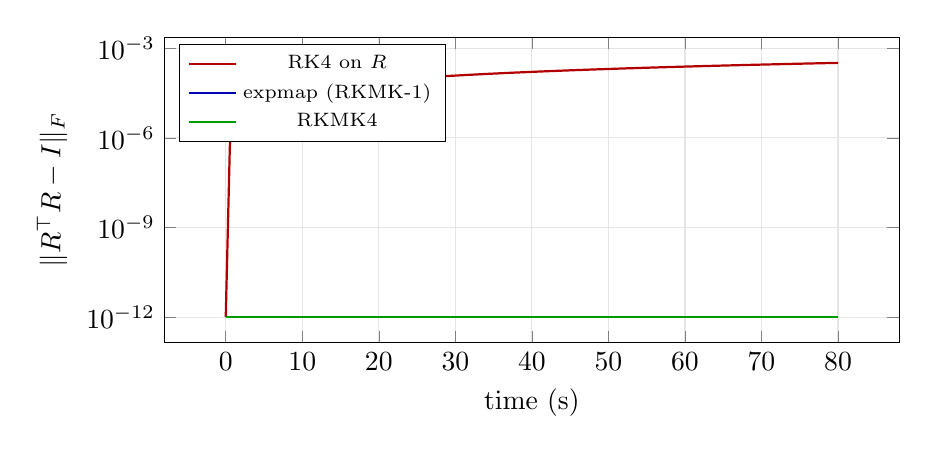
\begin{tikzpicture}
  \begin{axis}[
    width=0.9\linewidth,
    height=0.45\linewidth,
    xlabel={time (s)},
    ylabel={$\|R^\top R - I\|_F$},
    ymode=log,
    grid=both,
    grid style={gray!20},
    legend style={at={(0.02,0.98)},anchor=north west,font=\scriptsize},
  ]
    \addplot[thick,red!70!black] coordinates { (0.000,1.000000e-12) (0.600,2.415990e-06) (1.200,4.831976e-06) (1.800,7.247957e-06) (2.400,9.663935e-06) (3.000,1.207991e-05) (3.600,1.449588e-05) (4.200,1.691184e-05) (4.800,1.932780e-05) (5.400,2.174376e-05) (6.000,2.415971e-05) (6.600,2.657566e-05) (7.200,2.899161e-05) (7.800,3.140755e-05) (8.400,3.382348e-05) (9.000,3.623942e-05) (9.600,3.865534e-05) (10.200,4.107127e-05) (10.800,4.348719e-05) (11.400,4.590310e-05) (12.000,4.831901e-05) (12.600,5.073492e-05) (13.200,5.315082e-05) (13.800,5.556672e-05) (14.400,5.798262e-05) (15.000,6.039851e-05) (15.600,6.281440e-05) (16.200,6.523028e-05) (16.800,6.764616e-05) (17.400,7.006203e-05) (18.000,7.247790e-05) (18.600,7.489377e-05) (19.200,7.730963e-05) (19.800,7.972549e-05) (20.400,8.214134e-05) (21.000,8.455719e-05) (21.600,8.697304e-05) (22.200,8.938888e-05) (22.800,9.180472e-05) (23.400,9.422055e-05) (24.000,9.663638e-05) (24.600,9.905220e-05) (25.200,1.014680e-04) (25.800,1.038838e-04) (26.400,1.062997e-04) (27.000,1.087155e-04) (27.600,1.111313e-04) (28.200,1.135471e-04) (28.800,1.159629e-04) (29.400,1.183787e-04) (30.000,1.207944e-04) (30.600,1.232102e-04) (31.200,1.256260e-04) (31.800,1.280418e-04) (32.400,1.304575e-04) (33.000,1.328733e-04) (33.600,1.352891e-04) (34.200,1.377048e-04) (34.800,1.401206e-04) (35.400,1.425363e-04) (36.000,1.449521e-04) (36.600,1.473678e-04) (37.200,1.497836e-04) (37.800,1.521993e-04) (38.400,1.546150e-04) (39.000,1.570308e-04) (39.600,1.594465e-04) (40.200,1.618622e-04) (40.800,1.642779e-04) (41.400,1.666936e-04) (42.000,1.691093e-04) (42.600,1.715250e-04) (43.200,1.739407e-04) (43.800,1.763564e-04) (44.400,1.787721e-04) (45.000,1.811878e-04) (45.600,1.836035e-04) (46.200,1.860191e-04) (46.800,1.884348e-04) (47.400,1.908505e-04) (48.000,1.932662e-04) (48.600,1.956818e-04) (49.200,1.980975e-04) (49.800,2.005131e-04) (50.400,2.029288e-04) (51.000,2.053444e-04) (51.600,2.077600e-04) (52.200,2.101757e-04) (52.800,2.125913e-04) (53.400,2.150069e-04) (54.000,2.174226e-04) (54.600,2.198382e-04) (55.200,2.222538e-04) (55.800,2.246694e-04) (56.400,2.270850e-04) (57.000,2.295006e-04) (57.600,2.319162e-04) (58.200,2.343318e-04) (58.800,2.367474e-04) (59.400,2.391630e-04) (60.000,2.415786e-04) (60.600,2.439941e-04) (61.200,2.464097e-04) (61.800,2.488253e-04) (62.400,2.512408e-04) (63.000,2.536564e-04) (63.600,2.560720e-04) (64.200,2.584875e-04) (64.800,2.609031e-04) (65.400,2.633186e-04) (66.000,2.657341e-04) (66.600,2.681497e-04) (67.200,2.705652e-04) (67.800,2.729807e-04) (68.400,2.753963e-04) (69.000,2.778118e-04) (69.600,2.802273e-04) (70.200,2.826428e-04) (70.800,2.850583e-04) (71.400,2.874738e-04) (72.000,2.898893e-04) (72.600,2.923048e-04) (73.200,2.947203e-04) (73.800,2.971358e-04) (74.400,2.995513e-04) (75.000,3.019668e-04) (75.600,3.043822e-04) (76.200,3.067977e-04) (76.800,3.092132e-04) (77.400,3.116286e-04) (78.000,3.140441e-04) (78.600,3.164595e-04) (79.200,3.188750e-04) (79.800,3.212904e-04) (80.000,3.220956e-04) };
    \addlegendentry{RK4 on $R$}
    \addplot[thick,blue!70!black] coordinates { (0.000,1.000000e-12) (0.600,1.000000e-12) (1.200,1.000000e-12) (1.800,1.000000e-12) (2.400,1.000000e-12) (3.000,1.000000e-12) (3.600,1.000000e-12) (4.200,1.000000e-12) (4.800,1.000000e-12) (5.400,1.000000e-12) (6.000,1.000000e-12) (6.600,1.000000e-12) (7.200,1.000000e-12) (7.800,1.000000e-12) (8.400,1.000000e-12) (9.000,1.000000e-12) (9.600,1.000000e-12) (10.200,1.000000e-12) (10.800,1.000000e-12) (11.400,1.000000e-12) (12.000,1.000000e-12) (12.600,1.000000e-12) (13.200,1.000000e-12) (13.800,1.000000e-12) (14.400,1.000000e-12) (15.000,1.000000e-12) (15.600,1.000000e-12) (16.200,1.000000e-12) (16.800,1.000000e-12) (17.400,1.000000e-12) (18.000,1.000000e-12) (18.600,1.000000e-12) (19.200,1.000000e-12) (19.800,1.000000e-12) (20.400,1.000000e-12) (21.000,1.000000e-12) (21.600,1.000000e-12) (22.200,1.000000e-12) (22.800,1.000000e-12) (23.400,1.000000e-12) (24.000,1.000000e-12) (24.600,1.000000e-12) (25.200,1.000000e-12) (25.800,1.000000e-12) (26.400,1.000000e-12) (27.000,1.000000e-12) (27.600,1.000000e-12) (28.200,1.000000e-12) (28.800,1.000000e-12) (29.400,1.000000e-12) (30.000,1.000000e-12) (30.600,1.000000e-12) (31.200,1.000000e-12) (31.800,1.000000e-12) (32.400,1.000000e-12) (33.000,1.000000e-12) (33.600,1.000000e-12) (34.200,1.000000e-12) (34.800,1.000000e-12) (35.400,1.000000e-12) (36.000,1.000000e-12) (36.600,1.000000e-12) (37.200,1.000000e-12) (37.800,1.000000e-12) (38.400,1.000000e-12) (39.000,1.000000e-12) (39.600,1.000000e-12) (40.200,1.000000e-12) (40.800,1.000000e-12) (41.400,1.000000e-12) (42.000,1.000000e-12) (42.600,1.000000e-12) (43.200,1.000000e-12) (43.800,1.000000e-12) (44.400,1.000000e-12) (45.000,1.000000e-12) (45.600,1.000000e-12) (46.200,1.000000e-12) (46.800,1.000000e-12) (47.400,1.000000e-12) (48.000,1.000000e-12) (48.600,1.000000e-12) (49.200,1.000000e-12) (49.800,1.000000e-12) (50.400,1.000000e-12) (51.000,1.000000e-12) (51.600,1.000000e-12) (52.200,1.000000e-12) (52.800,1.000000e-12) (53.400,1.000000e-12) (54.000,1.000000e-12) (54.600,1.000000e-12) (55.200,1.000000e-12) (55.800,1.000000e-12) (56.400,1.000000e-12) (57.000,1.000000e-12) (57.600,1.000000e-12) (58.200,1.000000e-12) (58.800,1.000000e-12) (59.400,1.000000e-12) (60.000,1.000000e-12) (60.600,1.000000e-12) (61.200,1.000000e-12) (61.800,1.000000e-12) (62.400,1.000000e-12) (63.000,1.000000e-12) (63.600,1.000000e-12) (64.200,1.000000e-12) (64.800,1.000000e-12) (65.400,1.000000e-12) (66.000,1.000000e-12) (66.600,1.000000e-12) (67.200,1.000000e-12) (67.800,1.000000e-12) (68.400,1.000000e-12) (69.000,1.000000e-12) (69.600,1.000000e-12) (70.200,1.000000e-12) (70.800,1.000000e-12) (71.400,1.000000e-12) (72.000,1.000000e-12) (72.600,1.000000e-12) (73.200,1.000000e-12) (73.800,1.000000e-12) (74.400,1.000000e-12) (75.000,1.000000e-12) (75.600,1.000000e-12) (76.200,1.000000e-12) (76.800,1.000000e-12) (77.400,1.000000e-12) (78.000,1.000000e-12) (78.600,1.000000e-12) (79.200,1.000000e-12) (79.800,1.000000e-12) (80.000,1.000000e-12) };
    \addlegendentry{expmap (RKMK-1)}
    \addplot[thick,green!60!black] coordinates { (0.000,1.000000e-12) (0.600,1.000000e-12) (1.200,1.000000e-12) (1.800,1.000000e-12) (2.400,1.000000e-12) (3.000,1.000000e-12) (3.600,1.000000e-12) (4.200,1.000000e-12) (4.800,1.000000e-12) (5.400,1.000000e-12) (6.000,1.000000e-12) (6.600,1.000000e-12) (7.200,1.000000e-12) (7.800,1.000000e-12) (8.400,1.000000e-12) (9.000,1.000000e-12) (9.600,1.000000e-12) (10.200,1.000000e-12) (10.800,1.000000e-12) (11.400,1.000000e-12) (12.000,1.000000e-12) (12.600,1.000000e-12) (13.200,1.000000e-12) (13.800,1.000000e-12) (14.400,1.000000e-12) (15.000,1.000000e-12) (15.600,1.000000e-12) (16.200,1.000000e-12) (16.800,1.000000e-12) (17.400,1.000000e-12) (18.000,1.000000e-12) (18.600,1.000000e-12) (19.200,1.000000e-12) (19.800,1.000000e-12) (20.400,1.000000e-12) (21.000,1.000000e-12) (21.600,1.000000e-12) (22.200,1.000000e-12) (22.800,1.000000e-12) (23.400,1.000000e-12) (24.000,1.000000e-12) (24.600,1.000000e-12) (25.200,1.000000e-12) (25.800,1.000000e-12) (26.400,1.000000e-12) (27.000,1.000000e-12) (27.600,1.000000e-12) (28.200,1.000000e-12) (28.800,1.000000e-12) (29.400,1.000000e-12) (30.000,1.000000e-12) (30.600,1.000000e-12) (31.200,1.000000e-12) (31.800,1.000000e-12) (32.400,1.000000e-12) (33.000,1.000000e-12) (33.600,1.000000e-12) (34.200,1.000000e-12) (34.800,1.000000e-12) (35.400,1.000000e-12) (36.000,1.000000e-12) (36.600,1.000000e-12) (37.200,1.000000e-12) (37.800,1.000000e-12) (38.400,1.000000e-12) (39.000,1.000000e-12) (39.600,1.000000e-12) (40.200,1.000000e-12) (40.800,1.000000e-12) (41.400,1.000000e-12) (42.000,1.000000e-12) (42.600,1.000000e-12) (43.200,1.000000e-12) (43.800,1.000000e-12) (44.400,1.000000e-12) (45.000,1.000000e-12) (45.600,1.000000e-12) (46.200,1.000000e-12) (46.800,1.000000e-12) (47.400,1.000000e-12) (48.000,1.000000e-12) (48.600,1.000000e-12) (49.200,1.000000e-12) (49.800,1.000000e-12) (50.400,1.000000e-12) (51.000,1.000000e-12) (51.600,1.000000e-12) (52.200,1.000000e-12) (52.800,1.000000e-12) (53.400,1.000000e-12) (54.000,1.000000e-12) (54.600,1.000000e-12) (55.200,1.000000e-12) (55.800,1.000000e-12) (56.400,1.000000e-12) (57.000,1.000000e-12) (57.600,1.000000e-12) (58.200,1.000000e-12) (58.800,1.000000e-12) (59.400,1.000000e-12) (60.000,1.000000e-12) (60.600,1.000000e-12) (61.200,1.000000e-12) (61.800,1.000000e-12) (62.400,1.000000e-12) (63.000,1.000000e-12) (63.600,1.000000e-12) (64.200,1.000000e-12) (64.800,1.000000e-12) (65.400,1.000000e-12) (66.000,1.000000e-12) (66.600,1.000000e-12) (67.200,1.000000e-12) (67.800,1.000000e-12) (68.400,1.000000e-12) (69.000,1.000000e-12) (69.600,1.000000e-12) (70.200,1.000000e-12) (70.800,1.000000e-12) (71.400,1.000000e-12) (72.000,1.000000e-12) (72.600,1.000000e-12) (73.200,1.000000e-12) (73.800,1.000000e-12) (74.400,1.000000e-12) (75.000,1.000000e-12) (75.600,1.000000e-12) (76.200,1.000000e-12) (76.800,1.000000e-12) (77.400,1.000000e-12) (78.000,1.000000e-12) (78.600,1.000000e-12) (79.200,1.000000e-12) (79.800,1.000000e-12) (80.000,1.000000e-12) };
    \addlegendentry{RKMK4}
  \end{axis}
\end{tikzpicture}

  \caption{Orthonormality drift for RK4 on $\mathbf{R}$, expmap (RKMK-1), and
  RKMK4 at constant angular velocity.}
  \label{fig:integrator_drift}
\end{figure}
The same constant-rate setup can be compared to the exact solution
$\mathbf{R}_{\text{exact}}=\mathbf{R}_0\exp([\boldsymbol{\omega}\Delta t]_\times)$.
\Cref{fig:integrator_error} reports the error
$\|\mathbf{R}_{\text{est}}-\mathbf{R}_{\text{exact}}\|_F$ over time.
\begin{figure}[h]
  \centering
  % Auto-generated by latex/scripts/generate_figures.py
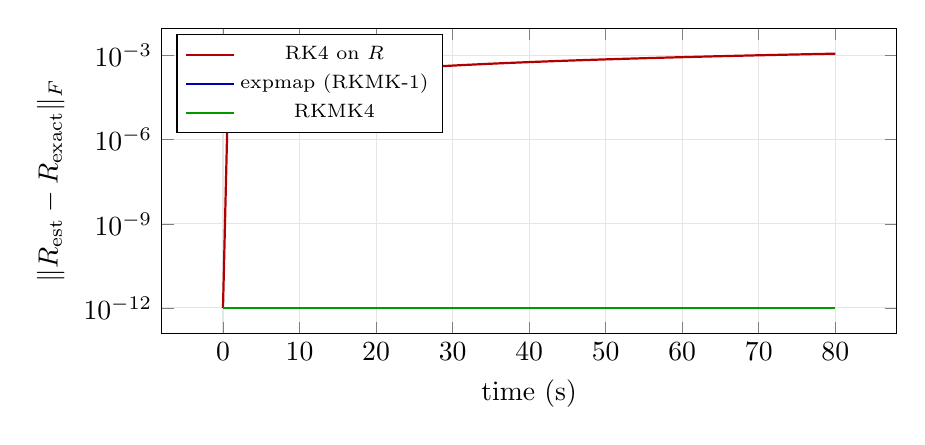
\begin{tikzpicture}
  \begin{axis}[
    width=0.9\linewidth,
    height=0.45\linewidth,
    xlabel={time (s)},
    ylabel={$\|R_{\text{est}}-R_{\text{exact}}\|_F$},
    ymode=log,
    grid=both,
    grid style={gray!20},
    legend style={at={(0.02,0.98)},anchor=north west,font=\scriptsize},
  ]
    \addplot[thick,red!70!black] coordinates { (0.000,1.000000e-12) (0.600,8.785029e-06) (1.200,1.757005e-05) (1.800,2.635507e-05) (2.400,3.514007e-05) (3.000,4.392507e-05) (3.600,5.271006e-05) (4.200,6.149505e-05) (4.800,7.028002e-05) (5.400,7.906499e-05) (6.000,8.784995e-05) (6.600,9.663491e-05) (7.200,1.054199e-04) (7.800,1.142048e-04) (8.400,1.229897e-04) (9.000,1.317746e-04) (9.600,1.405596e-04) (10.200,1.493445e-04) (10.800,1.581294e-04) (11.400,1.669143e-04) (12.000,1.756992e-04) (12.600,1.844840e-04) (13.200,1.932689e-04) (13.800,2.020538e-04) (14.400,2.108386e-04) (15.000,2.196235e-04) (15.600,2.284083e-04) (16.200,2.371932e-04) (16.800,2.459780e-04) (17.400,2.547628e-04) (18.000,2.635476e-04) (18.600,2.723324e-04) (19.200,2.811172e-04) (19.800,2.899020e-04) (20.400,2.986868e-04) (21.000,3.074716e-04) (21.600,3.162563e-04) (22.200,3.250411e-04) (22.800,3.338258e-04) (23.400,3.426106e-04) (24.000,3.513953e-04) (24.600,3.601800e-04) (25.200,3.689648e-04) (25.800,3.777495e-04) (26.400,3.865342e-04) (27.000,3.953189e-04) (27.600,4.041036e-04) (28.200,4.128883e-04) (28.800,4.216729e-04) (29.400,4.304576e-04) (30.000,4.392423e-04) (30.600,4.480269e-04) (31.200,4.568116e-04) (31.800,4.655962e-04) (32.400,4.743808e-04) (33.000,4.831655e-04) (33.600,4.919501e-04) (34.200,5.007347e-04) (34.800,5.095193e-04) (35.400,5.183039e-04) (36.000,5.270885e-04) (36.600,5.358730e-04) (37.200,5.446576e-04) (37.800,5.534422e-04) (38.400,5.622267e-04) (39.000,5.710113e-04) (39.600,5.797958e-04) (40.200,5.885804e-04) (40.800,5.973649e-04) (41.400,6.061494e-04) (42.000,6.149339e-04) (42.600,6.237184e-04) (43.200,6.325029e-04) (43.800,6.412874e-04) (44.400,6.500719e-04) (45.000,6.588564e-04) (45.600,6.676408e-04) (46.200,6.764253e-04) (46.800,6.852097e-04) (47.400,6.939942e-04) (48.000,7.027786e-04) (48.600,7.115630e-04) (49.200,7.203475e-04) (49.800,7.291319e-04) (50.400,7.379163e-04) (51.000,7.467007e-04) (51.600,7.554851e-04) (52.200,7.642695e-04) (52.800,7.730538e-04) (53.400,7.818382e-04) (54.000,7.906226e-04) (54.600,7.994069e-04) (55.200,8.081913e-04) (55.800,8.169756e-04) (56.400,8.257599e-04) (57.000,8.345443e-04) (57.600,8.433286e-04) (58.200,8.521129e-04) (58.800,8.608972e-04) (59.400,8.696815e-04) (60.000,8.784658e-04) (60.600,8.872500e-04) (61.200,8.960343e-04) (61.800,9.048186e-04) (62.400,9.136028e-04) (63.000,9.223871e-04) (63.600,9.311713e-04) (64.200,9.399556e-04) (64.800,9.487398e-04) (65.400,9.575240e-04) (66.000,9.663082e-04) (66.600,9.750924e-04) (67.200,9.838766e-04) (67.800,9.926608e-04) (68.400,1.001445e-03) (69.000,1.010229e-03) (69.600,1.019013e-03) (70.200,1.027797e-03) (70.800,1.036582e-03) (71.400,1.045366e-03) (72.000,1.054150e-03) (72.600,1.062934e-03) (73.200,1.071718e-03) (73.800,1.080502e-03) (74.400,1.089286e-03) (75.000,1.098070e-03) (75.600,1.106855e-03) (76.200,1.115639e-03) (76.800,1.124423e-03) (77.400,1.133207e-03) (78.000,1.141991e-03) (78.600,1.150775e-03) (79.200,1.159559e-03) (79.800,1.168343e-03) (80.000,1.171271e-03) };
    \addlegendentry{RK4 on $R$}
    \addplot[thick,blue!70!black] coordinates { (0.000,1.000000e-12) (0.600,1.000000e-12) (1.200,1.000000e-12) (1.800,1.000000e-12) (2.400,1.000000e-12) (3.000,1.000000e-12) (3.600,1.000000e-12) (4.200,1.000000e-12) (4.800,1.000000e-12) (5.400,1.000000e-12) (6.000,1.000000e-12) (6.600,1.000000e-12) (7.200,1.000000e-12) (7.800,1.000000e-12) (8.400,1.000000e-12) (9.000,1.000000e-12) (9.600,1.000000e-12) (10.200,1.000000e-12) (10.800,1.000000e-12) (11.400,1.000000e-12) (12.000,1.000000e-12) (12.600,1.000000e-12) (13.200,1.000000e-12) (13.800,1.000000e-12) (14.400,1.000000e-12) (15.000,1.000000e-12) (15.600,1.000000e-12) (16.200,1.000000e-12) (16.800,1.000000e-12) (17.400,1.000000e-12) (18.000,1.000000e-12) (18.600,1.000000e-12) (19.200,1.000000e-12) (19.800,1.000000e-12) (20.400,1.000000e-12) (21.000,1.000000e-12) (21.600,1.000000e-12) (22.200,1.000000e-12) (22.800,1.000000e-12) (23.400,1.000000e-12) (24.000,1.000000e-12) (24.600,1.000000e-12) (25.200,1.000000e-12) (25.800,1.000000e-12) (26.400,1.000000e-12) (27.000,1.000000e-12) (27.600,1.000000e-12) (28.200,1.000000e-12) (28.800,1.000000e-12) (29.400,1.000000e-12) (30.000,1.000000e-12) (30.600,1.000000e-12) (31.200,1.000000e-12) (31.800,1.000000e-12) (32.400,1.000000e-12) (33.000,1.000000e-12) (33.600,1.000000e-12) (34.200,1.000000e-12) (34.800,1.000000e-12) (35.400,1.000000e-12) (36.000,1.000000e-12) (36.600,1.000000e-12) (37.200,1.000000e-12) (37.800,1.000000e-12) (38.400,1.000000e-12) (39.000,1.000000e-12) (39.600,1.000000e-12) (40.200,1.000000e-12) (40.800,1.000000e-12) (41.400,1.000000e-12) (42.000,1.000000e-12) (42.600,1.000000e-12) (43.200,1.000000e-12) (43.800,1.000000e-12) (44.400,1.000000e-12) (45.000,1.000000e-12) (45.600,1.000000e-12) (46.200,1.000000e-12) (46.800,1.000000e-12) (47.400,1.000000e-12) (48.000,1.000000e-12) (48.600,1.000000e-12) (49.200,1.000000e-12) (49.800,1.000000e-12) (50.400,1.000000e-12) (51.000,1.000000e-12) (51.600,1.000000e-12) (52.200,1.000000e-12) (52.800,1.000000e-12) (53.400,1.000000e-12) (54.000,1.000000e-12) (54.600,1.000000e-12) (55.200,1.000000e-12) (55.800,1.000000e-12) (56.400,1.000000e-12) (57.000,1.000000e-12) (57.600,1.000000e-12) (58.200,1.000000e-12) (58.800,1.000000e-12) (59.400,1.000000e-12) (60.000,1.000000e-12) (60.600,1.000000e-12) (61.200,1.000000e-12) (61.800,1.000000e-12) (62.400,1.000000e-12) (63.000,1.000000e-12) (63.600,1.000000e-12) (64.200,1.000000e-12) (64.800,1.000000e-12) (65.400,1.000000e-12) (66.000,1.000000e-12) (66.600,1.000000e-12) (67.200,1.000000e-12) (67.800,1.000000e-12) (68.400,1.000000e-12) (69.000,1.000000e-12) (69.600,1.000000e-12) (70.200,1.000000e-12) (70.800,1.000000e-12) (71.400,1.000000e-12) (72.000,1.000000e-12) (72.600,1.000000e-12) (73.200,1.000000e-12) (73.800,1.000000e-12) (74.400,1.000000e-12) (75.000,1.000000e-12) (75.600,1.000000e-12) (76.200,1.000000e-12) (76.800,1.000000e-12) (77.400,1.000000e-12) (78.000,1.000000e-12) (78.600,1.000000e-12) (79.200,1.000000e-12) (79.800,1.000000e-12) (80.000,1.000000e-12) };
    \addlegendentry{expmap (RKMK-1)}
    \addplot[thick,green!60!black] coordinates { (0.000,1.000000e-12) (0.600,1.000000e-12) (1.200,1.000000e-12) (1.800,1.000000e-12) (2.400,1.000000e-12) (3.000,1.000000e-12) (3.600,1.000000e-12) (4.200,1.000000e-12) (4.800,1.000000e-12) (5.400,1.000000e-12) (6.000,1.000000e-12) (6.600,1.000000e-12) (7.200,1.000000e-12) (7.800,1.000000e-12) (8.400,1.000000e-12) (9.000,1.000000e-12) (9.600,1.000000e-12) (10.200,1.000000e-12) (10.800,1.000000e-12) (11.400,1.000000e-12) (12.000,1.000000e-12) (12.600,1.000000e-12) (13.200,1.000000e-12) (13.800,1.000000e-12) (14.400,1.000000e-12) (15.000,1.000000e-12) (15.600,1.000000e-12) (16.200,1.000000e-12) (16.800,1.000000e-12) (17.400,1.000000e-12) (18.000,1.000000e-12) (18.600,1.000000e-12) (19.200,1.000000e-12) (19.800,1.000000e-12) (20.400,1.000000e-12) (21.000,1.000000e-12) (21.600,1.000000e-12) (22.200,1.000000e-12) (22.800,1.000000e-12) (23.400,1.000000e-12) (24.000,1.000000e-12) (24.600,1.000000e-12) (25.200,1.000000e-12) (25.800,1.000000e-12) (26.400,1.000000e-12) (27.000,1.000000e-12) (27.600,1.000000e-12) (28.200,1.000000e-12) (28.800,1.000000e-12) (29.400,1.000000e-12) (30.000,1.000000e-12) (30.600,1.000000e-12) (31.200,1.000000e-12) (31.800,1.000000e-12) (32.400,1.000000e-12) (33.000,1.000000e-12) (33.600,1.000000e-12) (34.200,1.000000e-12) (34.800,1.000000e-12) (35.400,1.000000e-12) (36.000,1.000000e-12) (36.600,1.000000e-12) (37.200,1.000000e-12) (37.800,1.000000e-12) (38.400,1.000000e-12) (39.000,1.000000e-12) (39.600,1.000000e-12) (40.200,1.000000e-12) (40.800,1.000000e-12) (41.400,1.000000e-12) (42.000,1.000000e-12) (42.600,1.000000e-12) (43.200,1.000000e-12) (43.800,1.000000e-12) (44.400,1.000000e-12) (45.000,1.000000e-12) (45.600,1.000000e-12) (46.200,1.000000e-12) (46.800,1.000000e-12) (47.400,1.000000e-12) (48.000,1.000000e-12) (48.600,1.000000e-12) (49.200,1.000000e-12) (49.800,1.000000e-12) (50.400,1.000000e-12) (51.000,1.000000e-12) (51.600,1.000000e-12) (52.200,1.000000e-12) (52.800,1.000000e-12) (53.400,1.000000e-12) (54.000,1.000000e-12) (54.600,1.000000e-12) (55.200,1.000000e-12) (55.800,1.000000e-12) (56.400,1.000000e-12) (57.000,1.000000e-12) (57.600,1.000000e-12) (58.200,1.000000e-12) (58.800,1.000000e-12) (59.400,1.000000e-12) (60.000,1.000000e-12) (60.600,1.000000e-12) (61.200,1.000000e-12) (61.800,1.000000e-12) (62.400,1.000000e-12) (63.000,1.000000e-12) (63.600,1.000000e-12) (64.200,1.000000e-12) (64.800,1.000000e-12) (65.400,1.000000e-12) (66.000,1.000000e-12) (66.600,1.000000e-12) (67.200,1.000000e-12) (67.800,1.000000e-12) (68.400,1.000000e-12) (69.000,1.000000e-12) (69.600,1.000000e-12) (70.200,1.000000e-12) (70.800,1.000000e-12) (71.400,1.000000e-12) (72.000,1.000000e-12) (72.600,1.000000e-12) (73.200,1.000000e-12) (73.800,1.000000e-12) (74.400,1.000000e-12) (75.000,1.000000e-12) (75.600,1.000000e-12) (76.200,1.000000e-12) (76.800,1.000000e-12) (77.400,1.000000e-12) (78.000,1.000000e-12) (78.600,1.000000e-12) (79.200,1.000000e-12) (79.800,1.000000e-12) (80.000,1.000000e-12) };
    \addlegendentry{RKMK4}
  \end{axis}
\end{tikzpicture}

  \caption{Constant angular velocity: RK4, expmap (RKMK-1), and RKMK4 error
  relative to the exact solution.}
  \label{fig:integrator_error}
\end{figure}

\subsection{Example report: torque-free rigid-body tumble}
\textbf{Purpose.} Provide a verifiable nonlinear example with a reference
solution for error assessment.
\textbf{Definitions.} Inertia $\mathbf{I}$ is constant and diagonal; angular
velocity is body-frame.
\textbf{Assumptions.} Rigid body with constant inertia, no external torques,
body-frame angular velocity, and exact kinematics
$\dot{\mathbf{R}}=\mathbf{R}[\boldsymbol{\omega}]_\times$.
\textbf{Derivation.} Euler's rigid-body equations:
\begin{equation}
  \mathbf{I}\dot{\boldsymbol{\omega}} + \boldsymbol{\omega} \times (\mathbf{I}\boldsymbol{\omega}) = \mathbf{0}.
  \label{eq:tumble-omega}
\end{equation}
\textbf{Experiment.} Use $\mathbf{I}=\mathrm{diag}(3,2,1)$, initial
$\boldsymbol{\omega}(0)=[1.4,\,0.3,\,0.9]^\top$, and $\Delta t=0.01$~s for 60~s.
Integrate $\boldsymbol{\omega}$ with RK4. Update $\mathbf{R}$ either with RK4 on
$\dot{\mathbf{R}}$ (drift-prone) or with the expmap update
\Cref{eq:expmap-dq,eq:expmap-update} using the midpoint angular rate.
\textbf{Reference.} For error comparison, use a high-resolution expmap update
with $\Delta t_{\text{ref}}=0.001$~s (ten substeps per coarse step).
\textbf{Result.} \Cref{fig:integrator_tumbling} shows the orthonormality error
over time. RK4 on $\mathbf{R}$ drifts off $SO(3)$, while the expmap update
preserves orthonormality to numerical precision. \Cref{fig:integrator_tumbling_error}
shows the error relative to the reference solution.
\textbf{Implementation mapping.} The experiment and plots are generated by
\texttt{rigid\_body\_tumbling\_example()} in \texttt{latex/scripts/generate\_figures.py}.
\begin{figure}[h]
  \centering
  % Auto-generated by latex/scripts/generate_figures.py
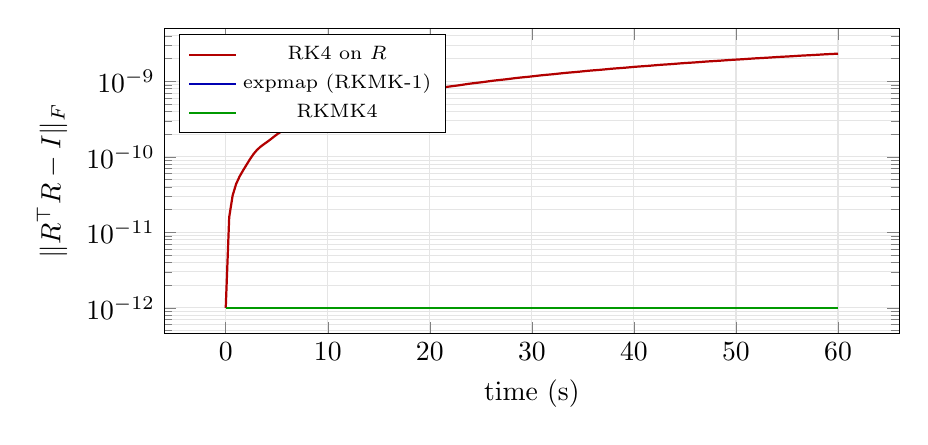
\begin{tikzpicture}
  \begin{axis}[
    width=0.9\linewidth,
    height=0.45\linewidth,
    xlabel={time (s)},
    ylabel={$\|R^\top R - I\|_F$},
    ymode=log,
    grid=both,
    grid style={gray!20},
    legend style={at={(0.02,0.98)},anchor=north west,font=\scriptsize},
  ]
    \addplot[thick,red!70!black] coordinates { (0.000,1.000000e-12) (0.340,1.594519e-11) (0.680,3.099969e-11) (1.020,4.387814e-11) (1.360,5.512156e-11) (1.700,6.623556e-11) (2.040,7.876740e-11) (2.380,9.339939e-11) (2.720,1.090311e-10) (3.060,1.235624e-10) (3.400,1.360605e-10) (3.740,1.472856e-10) (4.080,1.587424e-10) (4.420,1.718027e-10) (4.760,1.867757e-10) (5.100,2.022529e-10) (5.440,2.163072e-10) (5.780,2.284334e-10) (6.120,2.396201e-10) (6.460,2.513689e-10) (6.800,2.648652e-10) (7.140,2.800496e-10) (7.480,2.952831e-10) (7.820,3.088789e-10) (8.160,3.207128e-10) (8.500,3.319339e-10) (8.840,3.440000e-10) (9.180,3.578771e-10) (9.520,3.731568e-10) (9.860,3.880766e-10) (10.200,4.012465e-10) (10.540,4.128695e-10) (10.880,4.241903e-10) (11.220,4.365858e-10) (11.560,4.507780e-10) (11.900,4.660515e-10) (12.240,4.806204e-10) (12.580,4.934168e-10) (12.920,5.049060e-10) (13.260,5.163784e-10) (13.600,5.290980e-10) (13.940,5.435347e-10) (14.280,5.587196e-10) (14.620,5.729312e-10) (14.960,5.854149e-10) (15.300,5.968393e-10) (15.640,6.084954e-10) (15.980,6.215172e-10) (16.320,6.361298e-10) (16.660,6.511716e-10) (17.000,6.650405e-10) (17.340,6.772748e-10) (17.680,6.886871e-10) (18.020,7.005439e-10) (18.360,7.138415e-10) (18.700,7.285727e-10) (19.040,7.434384e-10) (19.380,7.569932e-10) (19.720,7.690329e-10) (20.060,7.804714e-10) (20.400,7.925347e-10) (20.740,8.060799e-10) (21.080,8.208879e-10) (21.420,8.355634e-10) (21.760,8.488399e-10) (22.100,8.607320e-10) (22.440,8.722212e-10) (22.780,8.844909e-10) (23.120,8.982626e-10) (23.460,9.131158e-10) (23.800,9.275980e-10) (24.140,9.406261e-10) (24.480,9.524006e-10) (24.820,9.639573e-10) (25.160,9.764370e-10) (25.500,9.904232e-10) (25.840,1.005303e-09) (26.180,1.019592e-09) (26.520,1.032394e-09) (26.860,1.044074e-09) (27.200,1.055714e-09) (27.540,1.068412e-09) (27.880,1.082607e-09) (28.220,1.097497e-09) (28.560,1.111591e-09) (28.900,1.124180e-09) (29.240,1.135780e-09) (29.580,1.147521e-09) (29.920,1.160455e-09) (30.260,1.174856e-09) (30.600,1.189736e-09) (30.940,1.203623e-09) (31.280,1.216002e-09) (31.620,1.227540e-09) (31.960,1.239408e-09) (32.300,1.252598e-09) (32.640,1.267201e-09) (32.980,1.282043e-09) (33.320,1.295703e-09) (33.660,1.307875e-09) (34.000,1.319373e-09) (34.340,1.331400e-09) (34.680,1.344870e-09) (35.020,1.359661e-09) (35.360,1.374422e-09) (35.700,1.387830e-09) (36.040,1.399804e-09) (36.380,1.411292e-09) (36.720,1.423519e-09) (37.060,1.437288e-09) (37.400,1.452235e-09) (37.740,1.466864e-09) (38.080,1.479996e-09) (38.420,1.491787e-09) (38.760,1.503306e-09) (39.100,1.515774e-09) (39.440,1.529849e-09) (39.780,1.544903e-09) (40.120,1.559339e-09) (40.460,1.572182e-09) (40.800,1.583819e-09) (41.140,1.595416e-09) (41.480,1.608164e-09) (41.820,1.622535e-09) (42.160,1.637631e-09) (42.500,1.651822e-09) (42.840,1.664374e-09) (43.180,1.675896e-09) (43.520,1.687621e-09) (43.860,1.700680e-09) (44.200,1.715316e-09) (44.540,1.730378e-09) (44.880,1.744277e-09) (45.220,1.756555e-09) (45.560,1.768007e-09) (45.900,1.779911e-09) (46.240,1.793295e-09) (46.580,1.808146e-09) (46.920,1.823098e-09) (47.260,1.836678e-09) (47.600,1.848709e-09) (47.940,1.860146e-09) (48.280,1.872272e-09) (48.620,1.885980e-09) (48.960,1.900982e-09) (49.300,1.915753e-09) (49.640,1.929006e-09) (49.980,1.940830e-09) (50.320,1.952302e-09) (50.660,1.964685e-09) (51.000,1.978699e-09) (51.340,1.993779e-09) (51.680,2.008314e-09) (52.020,2.021246e-09) (52.360,2.032910e-09) (52.700,2.044468e-09) (53.040,2.057130e-09) (53.380,2.071416e-09) (53.720,2.086503e-09) (54.060,2.100764e-09) (54.400,2.113397e-09) (54.740,2.124951e-09) (55.080,2.136637e-09) (55.420,2.149587e-09) (55.760,2.164104e-09) (56.100,2.179133e-09) (56.440,2.193099e-09) (56.780,2.205465e-09) (57.120,2.216957e-09) (57.460,2.228807e-09) (57.800,2.242046e-09) (58.140,2.256746e-09) (58.480,2.271662e-09) (58.820,2.285327e-09) (59.160,2.297463e-09) (59.500,2.308934e-09) (59.840,2.320976e-09) (60.000,2.327131e-09) };
    \addlegendentry{RK4 on $R$}
    \addplot[thick,blue!70!black] coordinates { (0.000,1.000000e-12) (0.340,1.000000e-12) (0.680,1.000000e-12) (1.020,1.000000e-12) (1.360,1.000000e-12) (1.700,1.000000e-12) (2.040,1.000000e-12) (2.380,1.000000e-12) (2.720,1.000000e-12) (3.060,1.000000e-12) (3.400,1.000000e-12) (3.740,1.000000e-12) (4.080,1.000000e-12) (4.420,1.000000e-12) (4.760,1.000000e-12) (5.100,1.000000e-12) (5.440,1.000000e-12) (5.780,1.000000e-12) (6.120,1.000000e-12) (6.460,1.000000e-12) (6.800,1.000000e-12) (7.140,1.000000e-12) (7.480,1.000000e-12) (7.820,1.000000e-12) (8.160,1.000000e-12) (8.500,1.000000e-12) (8.840,1.000000e-12) (9.180,1.000000e-12) (9.520,1.000000e-12) (9.860,1.000000e-12) (10.200,1.000000e-12) (10.540,1.000000e-12) (10.880,1.000000e-12) (11.220,1.000000e-12) (11.560,1.000000e-12) (11.900,1.000000e-12) (12.240,1.000000e-12) (12.580,1.000000e-12) (12.920,1.000000e-12) (13.260,1.000000e-12) (13.600,1.000000e-12) (13.940,1.000000e-12) (14.280,1.000000e-12) (14.620,1.000000e-12) (14.960,1.000000e-12) (15.300,1.000000e-12) (15.640,1.000000e-12) (15.980,1.000000e-12) (16.320,1.000000e-12) (16.660,1.000000e-12) (17.000,1.000000e-12) (17.340,1.000000e-12) (17.680,1.000000e-12) (18.020,1.000000e-12) (18.360,1.000000e-12) (18.700,1.000000e-12) (19.040,1.000000e-12) (19.380,1.000000e-12) (19.720,1.000000e-12) (20.060,1.000000e-12) (20.400,1.000000e-12) (20.740,1.000000e-12) (21.080,1.000000e-12) (21.420,1.000000e-12) (21.760,1.000000e-12) (22.100,1.000000e-12) (22.440,1.000000e-12) (22.780,1.000000e-12) (23.120,1.000000e-12) (23.460,1.000000e-12) (23.800,1.000000e-12) (24.140,1.000000e-12) (24.480,1.000000e-12) (24.820,1.000000e-12) (25.160,1.000000e-12) (25.500,1.000000e-12) (25.840,1.000000e-12) (26.180,1.000000e-12) (26.520,1.000000e-12) (26.860,1.000000e-12) (27.200,1.000000e-12) (27.540,1.000000e-12) (27.880,1.000000e-12) (28.220,1.000000e-12) (28.560,1.000000e-12) (28.900,1.000000e-12) (29.240,1.000000e-12) (29.580,1.000000e-12) (29.920,1.000000e-12) (30.260,1.000000e-12) (30.600,1.000000e-12) (30.940,1.000000e-12) (31.280,1.000000e-12) (31.620,1.000000e-12) (31.960,1.000000e-12) (32.300,1.000000e-12) (32.640,1.000000e-12) (32.980,1.000000e-12) (33.320,1.000000e-12) (33.660,1.000000e-12) (34.000,1.000000e-12) (34.340,1.000000e-12) (34.680,1.000000e-12) (35.020,1.000000e-12) (35.360,1.000000e-12) (35.700,1.000000e-12) (36.040,1.000000e-12) (36.380,1.000000e-12) (36.720,1.000000e-12) (37.060,1.000000e-12) (37.400,1.000000e-12) (37.740,1.000000e-12) (38.080,1.000000e-12) (38.420,1.000000e-12) (38.760,1.000000e-12) (39.100,1.000000e-12) (39.440,1.000000e-12) (39.780,1.000000e-12) (40.120,1.000000e-12) (40.460,1.000000e-12) (40.800,1.000000e-12) (41.140,1.000000e-12) (41.480,1.000000e-12) (41.820,1.000000e-12) (42.160,1.000000e-12) (42.500,1.000000e-12) (42.840,1.000000e-12) (43.180,1.000000e-12) (43.520,1.000000e-12) (43.860,1.000000e-12) (44.200,1.000000e-12) (44.540,1.000000e-12) (44.880,1.000000e-12) (45.220,1.000000e-12) (45.560,1.000000e-12) (45.900,1.000000e-12) (46.240,1.000000e-12) (46.580,1.000000e-12) (46.920,1.000000e-12) (47.260,1.000000e-12) (47.600,1.000000e-12) (47.940,1.000000e-12) (48.280,1.000000e-12) (48.620,1.000000e-12) (48.960,1.000000e-12) (49.300,1.000000e-12) (49.640,1.000000e-12) (49.980,1.000000e-12) (50.320,1.000000e-12) (50.660,1.000000e-12) (51.000,1.000000e-12) (51.340,1.000000e-12) (51.680,1.000000e-12) (52.020,1.000000e-12) (52.360,1.000000e-12) (52.700,1.000000e-12) (53.040,1.000000e-12) (53.380,1.000000e-12) (53.720,1.000000e-12) (54.060,1.000000e-12) (54.400,1.000000e-12) (54.740,1.000000e-12) (55.080,1.000000e-12) (55.420,1.000000e-12) (55.760,1.000000e-12) (56.100,1.000000e-12) (56.440,1.000000e-12) (56.780,1.000000e-12) (57.120,1.000000e-12) (57.460,1.000000e-12) (57.800,1.000000e-12) (58.140,1.000000e-12) (58.480,1.000000e-12) (58.820,1.000000e-12) (59.160,1.000000e-12) (59.500,1.000000e-12) (59.840,1.000000e-12) (60.000,1.000000e-12) };
    \addlegendentry{expmap (RKMK-1)}
    \addplot[thick,green!60!black] coordinates { (0.000,1.000000e-12) (0.340,1.000000e-12) (0.680,1.000000e-12) (1.020,1.000000e-12) (1.360,1.000000e-12) (1.700,1.000000e-12) (2.040,1.000000e-12) (2.380,1.000000e-12) (2.720,1.000000e-12) (3.060,1.000000e-12) (3.400,1.000000e-12) (3.740,1.000000e-12) (4.080,1.000000e-12) (4.420,1.000000e-12) (4.760,1.000000e-12) (5.100,1.000000e-12) (5.440,1.000000e-12) (5.780,1.000000e-12) (6.120,1.000000e-12) (6.460,1.000000e-12) (6.800,1.000000e-12) (7.140,1.000000e-12) (7.480,1.000000e-12) (7.820,1.000000e-12) (8.160,1.000000e-12) (8.500,1.000000e-12) (8.840,1.000000e-12) (9.180,1.000000e-12) (9.520,1.000000e-12) (9.860,1.000000e-12) (10.200,1.000000e-12) (10.540,1.000000e-12) (10.880,1.000000e-12) (11.220,1.000000e-12) (11.560,1.000000e-12) (11.900,1.000000e-12) (12.240,1.000000e-12) (12.580,1.000000e-12) (12.920,1.000000e-12) (13.260,1.000000e-12) (13.600,1.000000e-12) (13.940,1.000000e-12) (14.280,1.000000e-12) (14.620,1.000000e-12) (14.960,1.000000e-12) (15.300,1.000000e-12) (15.640,1.000000e-12) (15.980,1.000000e-12) (16.320,1.000000e-12) (16.660,1.000000e-12) (17.000,1.000000e-12) (17.340,1.000000e-12) (17.680,1.000000e-12) (18.020,1.000000e-12) (18.360,1.000000e-12) (18.700,1.000000e-12) (19.040,1.000000e-12) (19.380,1.000000e-12) (19.720,1.000000e-12) (20.060,1.000000e-12) (20.400,1.000000e-12) (20.740,1.000000e-12) (21.080,1.000000e-12) (21.420,1.000000e-12) (21.760,1.000000e-12) (22.100,1.000000e-12) (22.440,1.000000e-12) (22.780,1.000000e-12) (23.120,1.000000e-12) (23.460,1.000000e-12) (23.800,1.000000e-12) (24.140,1.000000e-12) (24.480,1.000000e-12) (24.820,1.000000e-12) (25.160,1.000000e-12) (25.500,1.000000e-12) (25.840,1.000000e-12) (26.180,1.000000e-12) (26.520,1.000000e-12) (26.860,1.000000e-12) (27.200,1.000000e-12) (27.540,1.000000e-12) (27.880,1.000000e-12) (28.220,1.000000e-12) (28.560,1.000000e-12) (28.900,1.000000e-12) (29.240,1.000000e-12) (29.580,1.000000e-12) (29.920,1.000000e-12) (30.260,1.000000e-12) (30.600,1.000000e-12) (30.940,1.000000e-12) (31.280,1.000000e-12) (31.620,1.000000e-12) (31.960,1.000000e-12) (32.300,1.000000e-12) (32.640,1.000000e-12) (32.980,1.000000e-12) (33.320,1.000000e-12) (33.660,1.000000e-12) (34.000,1.000000e-12) (34.340,1.000000e-12) (34.680,1.000000e-12) (35.020,1.000000e-12) (35.360,1.000000e-12) (35.700,1.000000e-12) (36.040,1.000000e-12) (36.380,1.000000e-12) (36.720,1.000000e-12) (37.060,1.000000e-12) (37.400,1.000000e-12) (37.740,1.000000e-12) (38.080,1.000000e-12) (38.420,1.000000e-12) (38.760,1.000000e-12) (39.100,1.000000e-12) (39.440,1.000000e-12) (39.780,1.000000e-12) (40.120,1.000000e-12) (40.460,1.000000e-12) (40.800,1.000000e-12) (41.140,1.000000e-12) (41.480,1.000000e-12) (41.820,1.000000e-12) (42.160,1.000000e-12) (42.500,1.000000e-12) (42.840,1.000000e-12) (43.180,1.000000e-12) (43.520,1.000000e-12) (43.860,1.000000e-12) (44.200,1.000000e-12) (44.540,1.000000e-12) (44.880,1.000000e-12) (45.220,1.000000e-12) (45.560,1.000000e-12) (45.900,1.000000e-12) (46.240,1.000000e-12) (46.580,1.000000e-12) (46.920,1.000000e-12) (47.260,1.000000e-12) (47.600,1.000000e-12) (47.940,1.000000e-12) (48.280,1.000000e-12) (48.620,1.000000e-12) (48.960,1.000000e-12) (49.300,1.000000e-12) (49.640,1.000000e-12) (49.980,1.000000e-12) (50.320,1.000000e-12) (50.660,1.000000e-12) (51.000,1.000000e-12) (51.340,1.000000e-12) (51.680,1.000000e-12) (52.020,1.000000e-12) (52.360,1.000000e-12) (52.700,1.000000e-12) (53.040,1.000000e-12) (53.380,1.000000e-12) (53.720,1.000000e-12) (54.060,1.000000e-12) (54.400,1.000000e-12) (54.740,1.000000e-12) (55.080,1.000000e-12) (55.420,1.000000e-12) (55.760,1.000000e-12) (56.100,1.000000e-12) (56.440,1.000000e-12) (56.780,1.000000e-12) (57.120,1.000000e-12) (57.460,1.000000e-12) (57.800,1.000000e-12) (58.140,1.000000e-12) (58.480,1.000000e-12) (58.820,1.000000e-12) (59.160,1.000000e-12) (59.500,1.000000e-12) (59.840,1.000000e-12) (60.000,1.000000e-12) };
    \addlegendentry{RKMK4}
  \end{axis}
\end{tikzpicture}

  \caption{Torque-free tumble: orthonormality drift for RK4 on $\mathbf{R}$,
  expmap (RKMK-1), and RKMK4.}
  \label{fig:integrator_tumbling}
\end{figure}
\begin{figure}[h]
  \centering
  % Auto-generated by latex/scripts/generate_figures.py
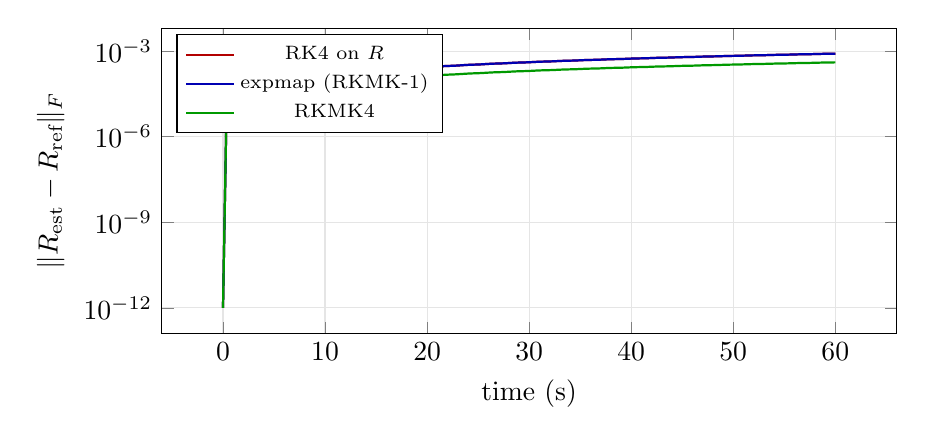
\begin{tikzpicture}
  \begin{axis}[
    width=0.9\linewidth,
    height=0.45\linewidth,
    xlabel={time (s)},
    ylabel={$\|R_{\text{est}}-R_{\text{ref}}\|_F$},
    ymode=log,
    grid=both,
    grid style={gray!20},
    legend style={at={(0.02,0.98)},anchor=north west,font=\scriptsize},
  ]
    \addplot[thick,red!70!black] coordinates { (0.000,1.000000e-12) (0.340,6.619174e-06) (0.680,1.271297e-05) (1.020,1.720473e-05) (1.360,2.020699e-05) (1.700,2.296877e-05) (2.040,2.701662e-05) (2.380,3.282767e-05) (2.720,3.941561e-05) (3.060,4.520610e-05) (3.400,4.930665e-05) (3.740,5.215892e-05) (4.080,5.515822e-05) (4.420,5.960776e-05) (4.760,6.567268e-05) (5.100,7.221021e-05) (5.440,7.768989e-05) (5.780,8.146226e-05) (6.120,8.423439e-05) (6.460,8.746295e-05) (6.800,9.225735e-05) (7.140,9.851473e-05) (7.480,1.049438e-04) (7.820,1.100950e-04) (8.160,1.135850e-04) (8.500,1.163441e-04) (8.840,1.198283e-04) (9.180,1.249418e-04) (9.520,1.313355e-04) (9.860,1.376020e-04) (10.200,1.424180e-04) (10.540,1.456758e-04) (10.880,1.484814e-04) (11.220,1.522408e-04) (11.560,1.576456e-04) (11.900,1.641200e-04) (12.240,1.701776e-04) (12.580,1.746649e-04) (12.920,1.777444e-04) (13.260,1.806470e-04) (13.600,1.846915e-04) (13.940,1.903566e-04) (14.280,1.968574e-04) (14.620,2.026696e-04) (14.960,2.068466e-04) (15.300,2.098015e-04) (15.640,2.128416e-04) (15.980,2.171742e-04) (16.320,2.230661e-04) (16.660,2.295411e-04) (17.000,2.350823e-04) (17.340,2.389765e-04) (17.680,2.418570e-04) (18.020,2.450662e-04) (18.360,2.496850e-04) (18.700,2.557684e-04) (19.040,2.621688e-04) (19.380,2.674240e-04) (19.720,2.710681e-04) (20.060,2.739189e-04) (20.400,2.773224e-04) (20.740,2.822228e-04) (21.080,2.884604e-04) (21.420,2.947418e-04) (21.760,2.997052e-04) (22.100,3.031336e-04) (22.440,3.059942e-04) (22.780,3.096138e-04) (23.120,3.147888e-04) (23.460,3.211412e-04) (23.800,3.272638e-04) (24.140,3.319367e-04) (24.480,3.351837e-04) (24.820,3.380899e-04) (25.160,3.419456e-04) (25.500,3.473854e-04) (25.840,3.538104e-04) (26.180,3.597392e-04) (26.520,3.641284e-04) (26.860,3.672272e-04) (27.200,3.702131e-04) (27.540,3.743245e-04) (27.880,3.800145e-04) (28.220,3.864675e-04) (28.560,3.921726e-04) (28.900,3.962883e-04) (29.240,3.992717e-04) (29.580,4.023723e-04) (29.920,4.067573e-04) (30.260,4.126769e-04) (30.600,4.191109e-04) (30.940,4.245669e-04) (31.280,4.284225e-04) (31.620,4.313250e-04) (31.960,4.345768e-04) (32.300,4.392497e-04) (32.640,4.453704e-04) (32.980,4.517373e-04) (33.320,4.569236e-04) (33.660,4.605359e-04) (34.000,4.633949e-04) (34.340,4.668355e-04) (34.680,4.718046e-04) (35.020,4.780897e-04) (35.360,4.843415e-04) (35.700,4.892423e-04) (36.040,4.926329e-04) (36.380,4.954902e-04) (36.720,4.991565e-04) (37.060,5.044213e-04) (37.400,5.108264e-04) (37.740,5.169162e-04) (38.080,5.215219e-04) (38.420,5.247186e-04) (38.760,5.276199e-04) (39.100,5.315450e-04) (39.440,5.370944e-04) (39.780,5.435688e-04) (40.120,5.494534e-04) (40.460,5.537614e-04) (40.800,5.567989e-04) (41.140,5.597924e-04) (41.480,5.640029e-04) (41.820,5.698147e-04) (42.160,5.763035e-04) (42.500,5.819446e-04) (42.840,5.859613e-04) (43.180,5.888812e-04) (43.520,5.920147e-04) (43.860,5.965281e-04) (44.200,6.025696e-04) (44.540,6.090162e-04) (44.880,6.143826e-04) (45.220,6.181238e-04) (45.560,6.209735e-04) (45.900,6.242918e-04) (46.240,6.291147e-04) (46.580,6.353443e-04) (46.920,6.416929e-04) (47.260,6.467625e-04) (47.600,6.502537e-04) (47.940,6.530837e-04) (48.280,6.566256e-04) (48.620,6.617538e-04) (48.960,6.681232e-04) (49.300,6.743213e-04) (49.640,6.790824e-04) (49.980,6.823578e-04) (50.320,6.852192e-04) (50.660,6.890157e-04) (51.000,6.944346e-04) (51.340,7.008909e-04) (51.680,7.068920e-04) (52.020,7.113439e-04) (52.360,7.144443e-04) (52.700,7.173860e-04) (53.040,7.214595e-04) (53.380,7.271456e-04) (53.720,7.336338e-04) (54.060,7.393991e-04) (54.400,7.435516e-04) (54.740,7.465221e-04) (55.080,7.495889e-04) (55.420,7.539531e-04) (55.760,7.598754e-04) (56.100,7.663409e-04) (56.440,7.718405e-04) (56.780,7.757128e-04) (57.120,7.785999e-04) (57.460,7.818314e-04) (57.800,7.864920e-04) (58.140,7.926136e-04) (58.480,7.990036e-04) (58.820,8.042176e-04) (59.160,8.078362e-04) (59.500,8.106862e-04) (59.840,8.141163e-04) (60.000,8.162385e-04) };
    \addlegendentry{RK4 on $R$}
    \addplot[thick,blue!70!black] coordinates { (0.000,1.000000e-12) (0.340,6.618703e-06) (0.680,1.271203e-05) (1.020,1.720335e-05) (1.360,2.020515e-05) (1.700,2.296644e-05) (2.040,2.701381e-05) (2.380,3.282439e-05) (2.720,3.941184e-05) (3.060,4.520185e-05) (3.400,4.930193e-05) (3.740,5.215373e-05) (4.080,5.515257e-05) (4.420,5.960166e-05) (4.760,6.566610e-05) (5.100,7.220314e-05) (5.440,7.768233e-05) (5.780,8.145422e-05) (6.120,8.422589e-05) (6.460,8.745400e-05) (6.800,9.224796e-05) (7.140,9.850485e-05) (7.480,1.049334e-04) (7.820,1.100841e-04) (8.160,1.135736e-04) (8.500,1.163323e-04) (8.840,1.198161e-04) (9.180,1.249291e-04) (9.520,1.313223e-04) (9.860,1.375883e-04) (10.200,1.424038e-04) (10.540,1.456611e-04) (10.880,1.484663e-04) (11.220,1.522252e-04) (11.560,1.576296e-04) (11.900,1.641035e-04) (12.240,1.701606e-04) (12.580,1.746473e-04) (12.920,1.777264e-04) (13.260,1.806286e-04) (13.600,1.846726e-04) (13.940,1.903373e-04) (14.280,1.968375e-04) (14.620,2.026493e-04) (14.960,2.068258e-04) (15.300,2.097802e-04) (15.640,2.128198e-04) (15.980,2.171520e-04) (16.320,2.230434e-04) (16.660,2.295179e-04) (17.000,2.350586e-04) (17.340,2.389523e-04) (17.680,2.418323e-04) (18.020,2.450411e-04) (18.360,2.496594e-04) (18.700,2.557423e-04) (19.040,2.621422e-04) (19.380,2.673969e-04) (19.720,2.710405e-04) (20.060,2.738909e-04) (20.400,2.772940e-04) (20.740,2.821939e-04) (21.080,2.884310e-04) (21.420,2.947119e-04) (21.760,2.996747e-04) (22.100,3.031027e-04) (22.440,3.059629e-04) (22.780,3.095820e-04) (23.120,3.147566e-04) (23.460,3.211084e-04) (23.800,3.272304e-04) (24.140,3.319029e-04) (24.480,3.351495e-04) (24.820,3.380552e-04) (25.160,3.419105e-04) (25.500,3.473497e-04) (25.840,3.537742e-04) (26.180,3.597025e-04) (26.520,3.640912e-04) (26.860,3.671896e-04) (27.200,3.701751e-04) (27.540,3.742860e-04) (27.880,3.799756e-04) (28.220,3.864280e-04) (28.560,3.921325e-04) (28.900,3.962478e-04) (29.240,3.992308e-04) (29.580,4.023310e-04) (29.920,4.067154e-04) (30.260,4.126346e-04) (30.600,4.190680e-04) (30.940,4.245235e-04) (31.280,4.283787e-04) (31.620,4.312807e-04) (31.960,4.345321e-04) (32.300,4.392045e-04) (32.640,4.453247e-04) (32.980,4.516911e-04) (33.320,4.568768e-04) (33.660,4.604887e-04) (34.000,4.633473e-04) (34.340,4.667875e-04) (34.680,4.717561e-04) (35.020,4.780407e-04) (35.360,4.842919e-04) (35.700,4.891922e-04) (36.040,4.925824e-04) (36.380,4.954393e-04) (36.720,4.991051e-04) (37.060,5.043694e-04) (37.400,5.107739e-04) (37.740,5.168633e-04) (38.080,5.214685e-04) (38.420,5.246648e-04) (38.760,5.275656e-04) (39.100,5.314903e-04) (39.440,5.370391e-04) (39.780,5.435130e-04) (40.120,5.493971e-04) (40.460,5.537047e-04) (40.800,5.567418e-04) (41.140,5.597348e-04) (41.480,5.639448e-04) (41.820,5.697561e-04) (42.160,5.762444e-04) (42.500,5.818850e-04) (42.840,5.859012e-04) (43.180,5.888208e-04) (43.520,5.919538e-04) (43.860,5.964667e-04) (44.200,6.025077e-04) (44.540,6.089538e-04) (44.880,6.143197e-04) (45.220,6.180604e-04) (45.560,6.209097e-04) (45.900,6.242276e-04) (46.240,6.290500e-04) (46.580,6.352791e-04) (46.920,6.416272e-04) (47.260,6.466963e-04) (47.600,6.501870e-04) (47.940,6.530166e-04) (48.280,6.565581e-04) (48.620,6.616858e-04) (48.960,6.680546e-04) (49.300,6.742522e-04) (49.640,6.790129e-04) (49.980,6.822878e-04) (50.320,6.851488e-04) (50.660,6.889449e-04) (51.000,6.943632e-04) (51.340,7.008190e-04) (51.680,7.068196e-04) (52.020,7.112710e-04) (52.360,7.143710e-04) (52.700,7.173123e-04) (53.040,7.213853e-04) (53.380,7.270709e-04) (53.720,7.335586e-04) (54.060,7.393234e-04) (54.400,7.434754e-04) (54.740,7.464454e-04) (55.080,7.495118e-04) (55.420,7.538755e-04) (55.760,7.597973e-04) (56.100,7.662623e-04) (56.440,7.717615e-04) (56.780,7.756333e-04) (57.120,7.785200e-04) (57.460,7.817510e-04) (57.800,7.864112e-04) (58.140,7.925322e-04) (58.480,7.989217e-04) (58.820,8.041352e-04) (59.160,8.077533e-04) (59.500,8.106029e-04) (59.840,8.140326e-04) (60.000,8.161545e-04) };
    \addlegendentry{expmap (RKMK-1)}
    \addplot[thick,green!60!black] coordinates { (0.000,1.000000e-12) (0.340,7.415579e-06) (0.680,1.307317e-05) (1.020,1.573877e-05) (1.360,1.572202e-05) (1.700,1.432653e-05) (2.040,1.379528e-05) (2.380,1.646704e-05) (2.720,2.128694e-05) (3.060,2.533039e-05) (3.400,2.727311e-05) (3.740,2.765864e-05) (4.080,2.790088e-05) (4.420,2.946620e-05) (4.760,3.288016e-05) (5.100,3.698711e-05) (5.440,4.007754e-05) (5.780,4.159749e-05) (6.120,4.228631e-05) (6.460,4.334389e-05) (6.800,4.567139e-05) (7.140,4.920574e-05) (7.480,5.281628e-05) (7.820,5.535378e-05) (8.160,5.671432e-05) (8.500,5.769534e-05) (8.840,5.927081e-05) (9.180,6.196529e-05) (9.520,6.543015e-05) (9.860,6.864525e-05) (10.200,7.085413e-05) (10.540,7.220374e-05) (10.880,7.345739e-05) (11.220,7.538239e-05) (11.560,7.824233e-05) (11.900,8.156116e-05) (12.240,8.447642e-05) (12.580,8.650925e-05) (12.920,8.792402e-05) (13.260,8.940786e-05) (13.600,9.155623e-05) (13.940,9.446274e-05) (14.280,9.762420e-05) (14.620,1.003362e-04) (14.960,1.022938e-04) (15.300,1.037972e-04) (15.640,1.054522e-04) (15.980,1.077266e-04) (16.320,1.106194e-04) (16.660,1.136546e-04) (17.000,1.162482e-04) (17.340,1.181844e-04) (17.680,1.197624e-04) (18.020,1.215258e-04) (18.360,1.238605e-04) (18.700,1.267271e-04) (19.040,1.296879e-04) (19.380,1.322223e-04) (19.720,1.341497e-04) (20.060,1.357671e-04) (20.400,1.375855e-04) (20.740,1.399502e-04) (21.080,1.428131e-04) (21.420,1.457508e-04) (21.760,1.482518e-04) (22.100,1.501526e-04) (22.440,1.517688e-04) (22.780,1.536092e-04) (23.120,1.560075e-04) (23.460,1.589073e-04) (23.800,1.618551e-04) (24.140,1.643153e-04) (24.480,1.661555e-04) (24.820,1.677384e-04) (25.160,1.695943e-04) (25.500,1.720564e-04) (25.840,1.750333e-04) (26.180,1.779957e-04) (26.520,1.803832e-04) (26.860,1.821272e-04) (27.200,1.836633e-04) (27.540,1.855550e-04) (27.880,1.881245e-04) (28.220,1.912015e-04) (28.560,1.941536e-04) (28.900,1.964247e-04) (29.240,1.980484e-04) (29.580,1.995476e-04) (29.920,2.015159e-04) (30.260,2.042343e-04) (30.600,2.074075e-04) (30.940,2.103019e-04) (31.280,2.124153e-04) (31.620,2.139141e-04) (31.960,2.154090e-04) (32.300,2.175043e-04) (32.640,2.203968e-04) (32.980,2.236333e-04) (33.320,2.264126e-04) (33.660,2.283416e-04) (34.000,2.297339e-04) (34.340,2.312735e-04) (34.680,2.335431e-04) (35.020,2.366091e-04) (35.360,2.398531e-04) (35.700,2.424645e-04) (36.040,2.442039e-04) (36.380,2.455285e-04) (36.720,2.471688e-04) (37.060,2.496449e-04) (37.400,2.528552e-04) (37.740,2.560404e-04) (38.080,2.584469e-04) (38.420,2.600151e-04) (38.760,2.613248e-04) (39.100,2.631177e-04) (39.440,2.658088e-04) (39.780,2.691114e-04) (40.120,2.721745e-04) (40.460,2.743623e-04) (40.800,2.757972e-04) (41.140,2.771496e-04) (41.480,2.791332e-04) (41.820,2.820220e-04) (42.160,2.853521e-04) (42.500,2.882448e-04) (42.840,2.902242e-04) (43.180,2.915764e-04) (43.520,2.930240e-04) (43.860,2.952159e-04) (44.200,2.982634e-04) (44.540,3.015564e-04) (44.880,3.042528e-04) (45.220,3.060535e-04) (45.560,3.073770e-04) (45.900,3.089599e-04) (46.240,3.113558e-04) (46.580,3.145098e-04) (46.920,3.177127e-04) (47.260,3.202099e-04) (47.600,3.218738e-04) (47.940,3.232171e-04) (48.280,3.249580e-04) (48.620,3.275350e-04) (48.960,3.307411e-04) (49.300,3.338198e-04) (49.640,3.361340e-04) (49.980,3.377053e-04) (50.320,3.391054e-04) (50.660,3.410094e-04) (51.000,3.437334e-04) (51.340,3.469450e-04) (51.680,3.498855e-04) (52.020,3.520439e-04) (52.360,3.535618e-04) (52.700,3.550413e-04) (53.040,3.570992e-04) (53.380,3.599335e-04) (53.720,3.631185e-04) (54.060,3.659231e-04) (54.400,3.679552e-04) (54.740,3.694484e-04) (55.080,3.710161e-04) (55.420,3.732109e-04) (55.760,3.761248e-04) (56.100,3.792664e-04) (56.440,3.819464e-04) (56.780,3.838765e-04) (57.120,3.853617e-04) (57.460,3.870170e-04) (57.800,3.893311e-04) (58.140,3.923043e-04) (58.480,3.953979e-04) (58.820,3.979655e-04) (59.160,3.998086e-04) (59.500,4.012930e-04) (59.840,4.030312e-04) (60.000,4.040764e-04) };
    \addlegendentry{RKMK4}
  \end{axis}
\end{tikzpicture}

  \caption{Torque-free tumble: RK4, expmap (RKMK-1), and RKMK4 error relative to
  a high-resolution expmap reference solution.}
  \label{fig:integrator_tumbling_error}
\end{figure}

\section{Applying integrators to the Fossen 6~DOF model}
\label{app:fossen-map}
The simulator state is
\[
  \mathbf{x}_6 =
  \begin{bmatrix}
    \mathbf{p} \\
    \mathbf{q}_{WB} \\
    \boldsymbol{\nu}
  \end{bmatrix},
  \quad
  \boldsymbol{\nu}=
  \begin{bmatrix}
    \mathbf{v} \\
    \boldsymbol{\omega}
  \end{bmatrix},
\]
with kinematics and dynamics:
\begin{align}
  \dot{\mathbf{p}} &= \mathbf{R}(\mathbf{q}_{WB})\mathbf{v}, \label{eq:fossen-kin-p} \\
  \dot{\mathbf{q}}_{WB} &= \tfrac{1}{2}\boldsymbol{\Omega}(\boldsymbol{\omega})\mathbf{q}_{WB}, \label{eq:fossen-kin-q} \\
  \dot{\boldsymbol{\nu}} &=
  \mathbf{M}^{-1}\!\Big(
    \boldsymbol{\tau}+\boldsymbol{\tau}_{\mathrm{env}}
    - \mathbf{C}_{RB}(\boldsymbol{\nu})\boldsymbol{\nu}
    - \mathbf{C}_{A}(\boldsymbol{\nu}_r)\boldsymbol{\nu}_r
    - \mathbf{D}(\boldsymbol{\nu}_r)\boldsymbol{\nu}_r
    - \mathbf{g}(\boldsymbol{\eta})
    + \mathbf{M}_A \dot{\boldsymbol{\nu}}_c
  \Big).
  \label{eq:fossen-dyn}
\end{align}

\paragraph{Equation-by-equation mapping to code}
\begin{itemize}
  \item \Cref{eq:fossen-kin-p,eq:fossen-kin-q} are implemented in
    \texttt{Fossen6DOF.kinematics()} using \texttt{rotation\_matrix\_from\_quaternion\_wxyz()}
    and \texttt{quaternion\_derivative\_wxyz()}.
  \item \Cref{eq:fossen-dyn} is implemented in \texttt{Fossen6DOF.dynamics()} with
    $\mathbf{C}_{RB}$ and $\mathbf{C}_A$ built by \texttt{coriolis\_from\_mass\_matrix()},
    and damping $\mathbf{D}$ from diagonal linear and quadratic terms in
    \texttt{Fossen6DOF.damping()}.
  \item Restoring forces $\mathbf{g}(\boldsymbol{\eta})$ use
    \texttt{restoring\_forces\_body()} with $\mathbf{R}^\top(\mathbf{q}_{WB})$.
  \item The full state derivative is assembled in
    \texttt{Fossen6DOF.state\_derivative()}.
  \item Integration uses \Cref{eq:euler} or \Cref{eq:rk4} in
    \texttt{Fossen6DOF.step()} for \texttt{euler} and \texttt{rk4} modes.
  \item The \texttt{expmap} mode uses \Cref{eq:rk4} for $\mathbf{p}$ and
    $\boldsymbol{\nu}$, and \Cref{eq:expmap-dq,eq:expmap-update} for attitude
    using the RK4-averaged angular rate.
\end{itemize}

\end{document}
